\section{Can I already play the that song that I like?}

The answer is, "kinda". So far you've made your first sounds and played along with a known song.

By just reading tabs you can get quite far. But you will most likely be stuck with playing along with songs without really knowing what is going on. And \textbf{if that is your goal, that is completely fine}.

However, by getting familiar with the fretboard (which frets are which notes, and how to check this), you can be a lot more creative with music.

Later on you will also learn about scales, which allow to you improvise over songs. To know which frets (or chords) to play, you will need to know which notes belong to the frets.

Additionally, some (mostly classical) music doesn't have a version with tabs. Meaning that reading notes is still good to know.

\section{Music staff}

You have already seen the music staff from \autoref{fig:music_note_names_on_staff} in the previous exercises. But the meaning of it was not explained yet.

\begin{itemize}
	\item The letters A-G on the staff show which line on the staff has which note name. Notes names go from A to G as shown in an earlier chapter.
	\item The notes go up alphabetically (starting again with A after G). 
	\item Notes in between the lines nicely spell out \textbf{"FACE"}, making it easy to remember.
	\item Note on the lines can be remembered with the mnemonic "\textbf{E}very \textbf{G}ood \textbf{B}oy \textbf{D}oes \textbf{F}ine".
	\item The most left symbol (\clefG) is called the G clef. Note that the curl of the G clef is on the line of the G note (second line from the bottom). 
	\item The vertical line in the middle indicates the start/end of a measure.
	\item The thicker vertical line in at the end indicates the end of the piece.
\end{itemize}

\begin{figure}[h]
	\centering
	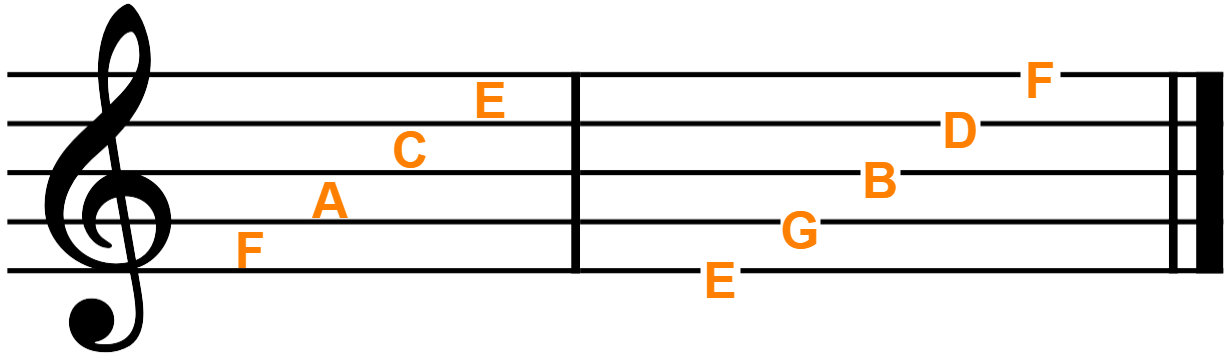
\includegraphics[width=0.6\textwidth]{../../Images/MusicNotation_MeasureNoteNames.png}
	\caption{Note names on the staff in two measures}
	\label{fig:music_note_names_on_staff}
\end{figure}

Detail: note that the clef shown in \autoref{fig:music_note_names_on_staff} is different than the ones seen in earlier exercises. For guitar notation you sometimes see a little 8 under the clef. This means that the original position of "middle C" (C4) with treble clef sounds an octave lower. This Results in the C that you see in \autoref{fig:music_note_names_on_staff} to be the middle C (C4) when there is a little 8 below the clef.

\newpage

\section{Counting}

So far we have also only seen one type of note. The quarter note. However, there are more. See \autoref{fig:note_duration_basic}. The \lilyTimeSignature{4}{4} means that there can fit 4 (top number) quarter notes (bottom number) in a measure. 

\begin{figure}[h]
	\centering
	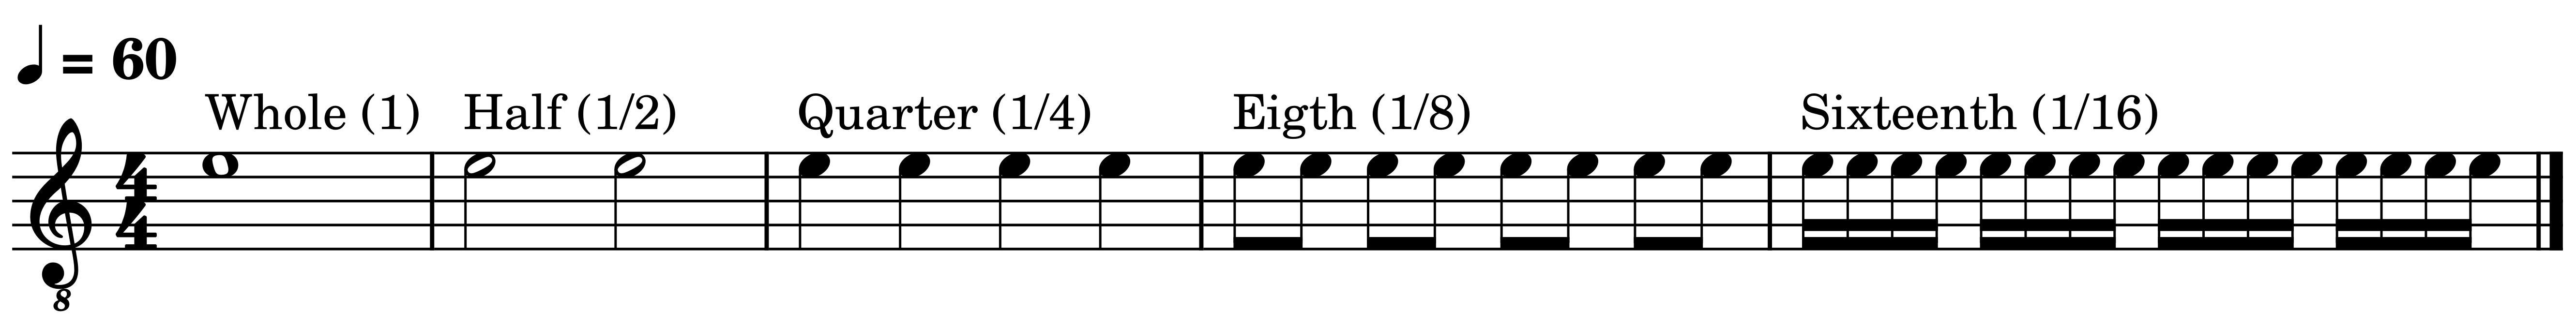
\includegraphics[width=\textwidth]{../../MuseScore/Guitar/MusicNotation/NoteDurations_Basic.png}
	\caption{Note duration}
	\label{fig:note_duration_basic}
\end{figure}

\textbf{Important}: A whole note (\wholeNote) equal 4 quarter notes (\quarterNote). It does \textbf{not} equal a whole measure. \newline

There are also other time signatures. The top value indicates how many notes of the bottom number's duration fit in a measure. So a \lilyTimeSignature{3}{4} time signature can fit 3 quarter notes per measure. And a \lilyTimeSignature{6}{8} time signature can fit 6 eighth notes per measure. Note that \lilyTimeSignature{3}{4} and \lilyTimeSignature{6}{8} indicate the same duration per measure, but they provide a different feel. This is demonstrated in \autoref{fig:time_signatures}.

In \autoref{fig:time_signatures} you also see a new duration notation. In the first measure with \lilyTimeSignature{6}{8} timing, there are dots next to the notes (\quarterNoteDottedDown). This means that the note has a duration of 1.5x its original duration.

The ">" symbol means that this note should be played with a more powerful accent. The \textbf{bold} numbers above the notes indicate the counting of the notes. A bold number means to put an accent on it, but played less accented then the ones where there is also an ">" symbol.

\begin{figure}[h]
	\centering
	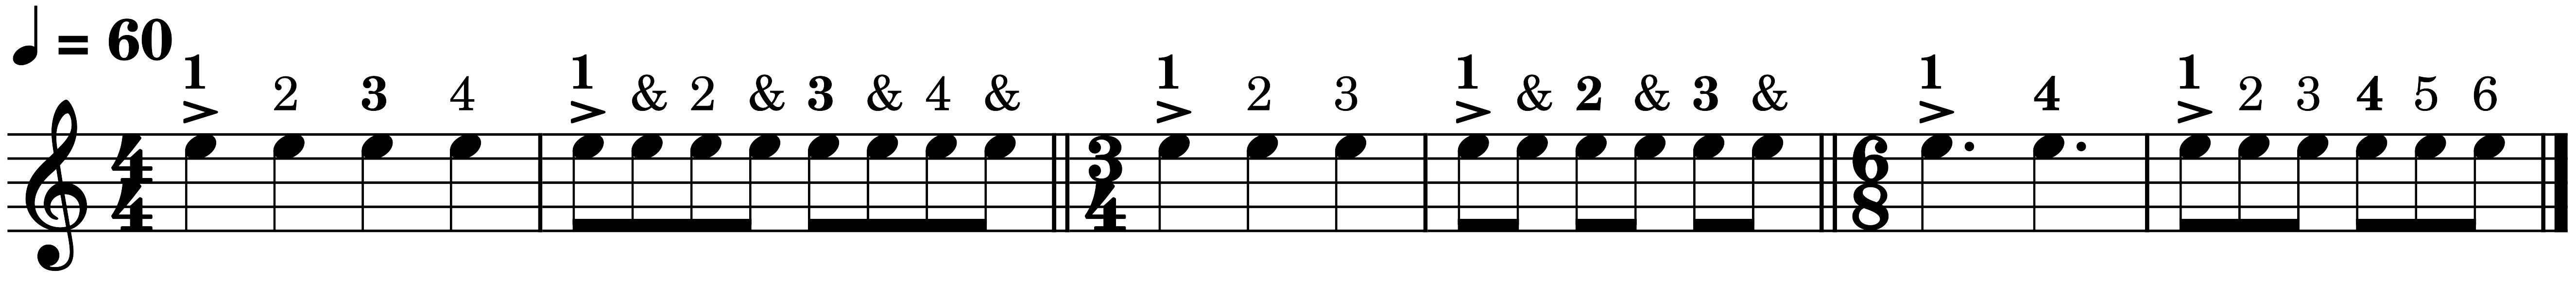
\includegraphics[width=\textwidth]{../../MuseScore/Guitar/MusicNotation/TimeSignature.png}
	\caption{Time signatures}
	\label{fig:time_signatures}
\end{figure}

Remember exercise \autoref{fig:exercise_nothing_else_matters_metallica_intro_pima} (Metallica - Nothing else matters (intro))? That is also in \lilyTimeSignature{6}{8}.

\newpage

Where notes indicate when to play a sound, rests indicate when to be silent. In \autoref{fig:guitar_rests} the most common rest durations are shown.

\begin{figure}[h]
	\centering
	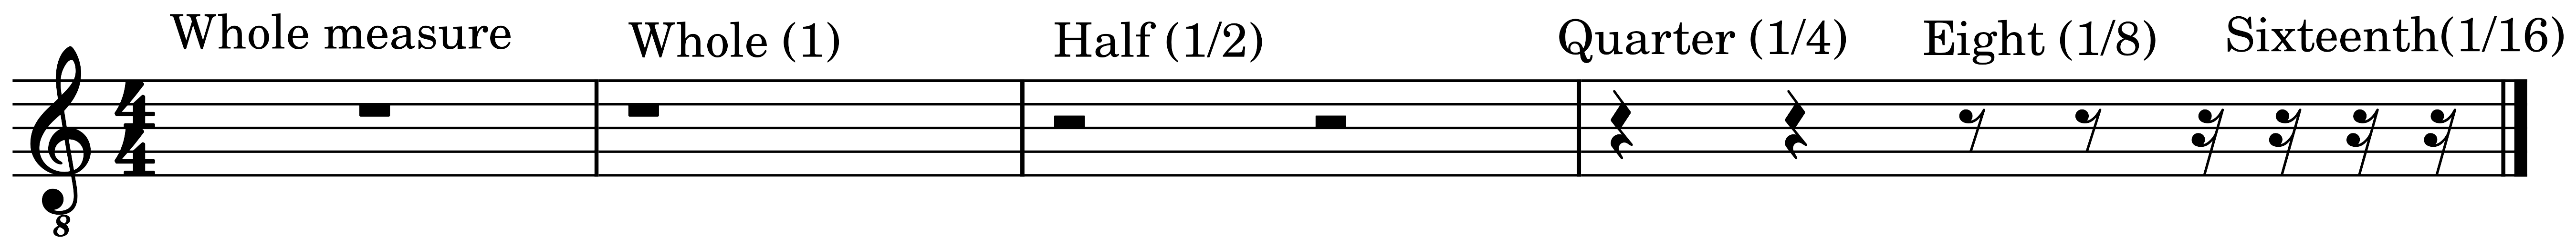
\includegraphics[width=\textwidth]{../../MuseScore/Guitar/GuitarRests.png}
	\caption{Rest notations of different duration}
	\label{fig:guitar_rests}
\end{figure}

In \autoref{fig:guitar_rests_exercise} an exercise is provided to count the rests. Remember to take this slow and to be conscious about the counts. As a help the tempo is set to the 60 quarter notes per minutes (BPM). This way each quarter note is 1 second. But feel free to play it slower.

\begin{figure}[h]
	\centering
	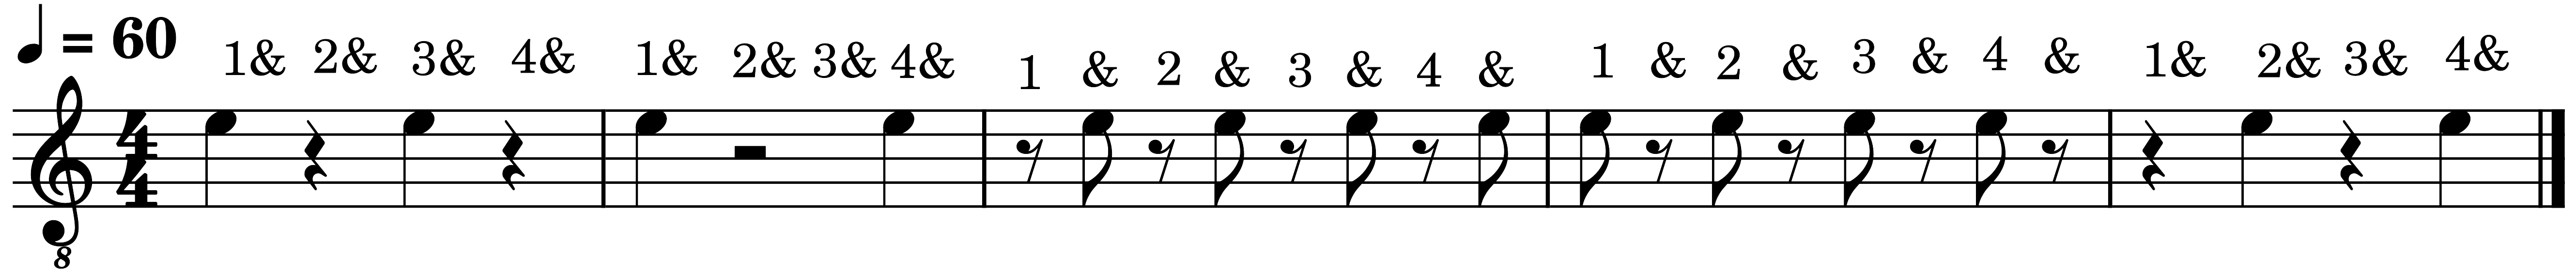
\includegraphics[width=\textwidth]{../../MuseScore/Guitar/GuitarRestsExercise.png}
	\caption{Rest notations of different duration}
	\label{fig:guitar_rests_exercise}
\end{figure}


\newpage

\section{Learning the main notes} \label{sec:learning_main_notes}

As a first tune that uses multiple note durations, and to learn the first notes on the guitar, Jingle bells will be played (\autoref{fig:jingle_bells}). The notes used for this tune are shown in \autoref{fig:notes_in_jingle_bells}.

\begin{figure}[h]
	\centering
	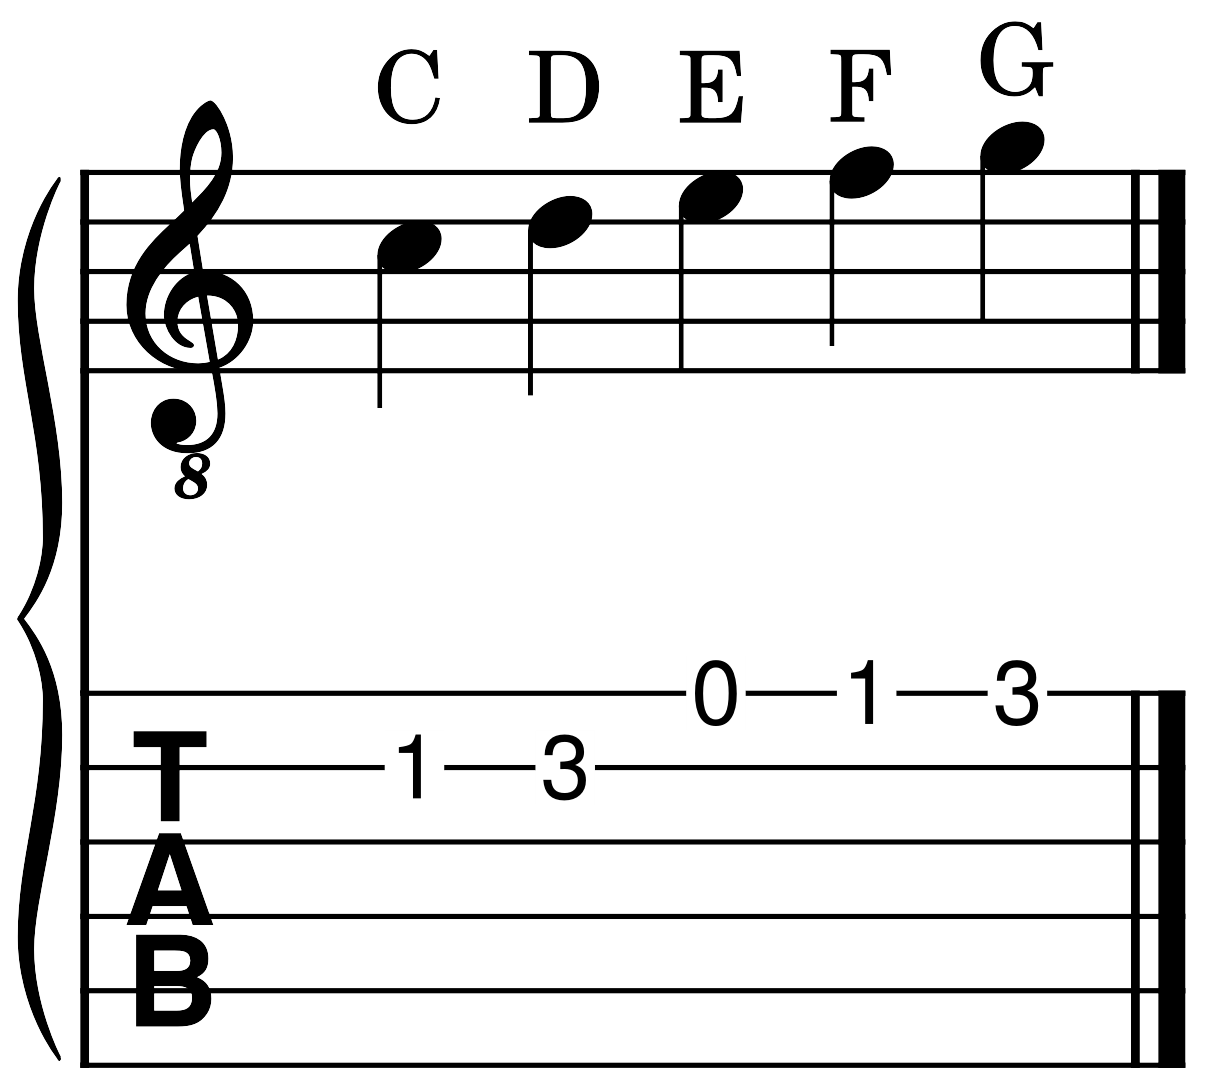
\includegraphics[height=0.12\textheight]{../../MuseScore/Guitar/NotesInJingleBells.png}
	\caption{Notes used in jingle bells}
	\label{fig:notes_in_jingle_bells}
\end{figure}

Now Jingle bells can be played as shown in \autoref{fig:jingle_bells}.

\begin{figure}[h]
	\centering
	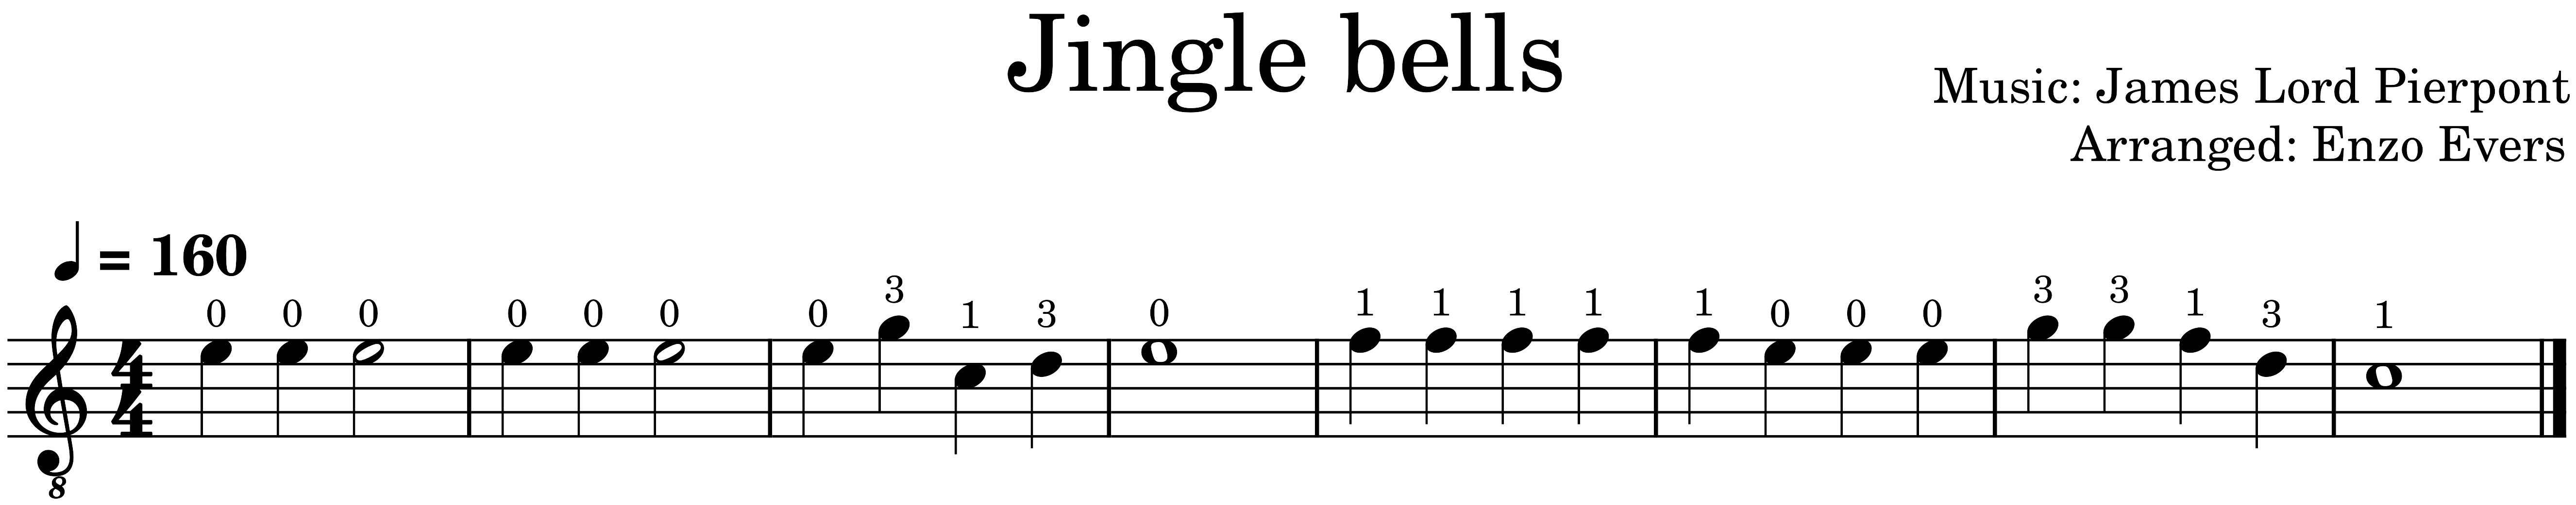
\includegraphics[width=\textwidth]{../../MuseScore/Guitar/GuitarJingleBells.png}
	\caption{Jingle bells}
	\label{fig:jingle_bells}
\end{figure}

\newpage

To learn a few more notes, the "Tetris" tune will be played. The notes from \autoref{fig:notes_for_tetris_first_part} should are used in this tune. The only new notes are A and B.

\begin{figure}[h]
	\centering
	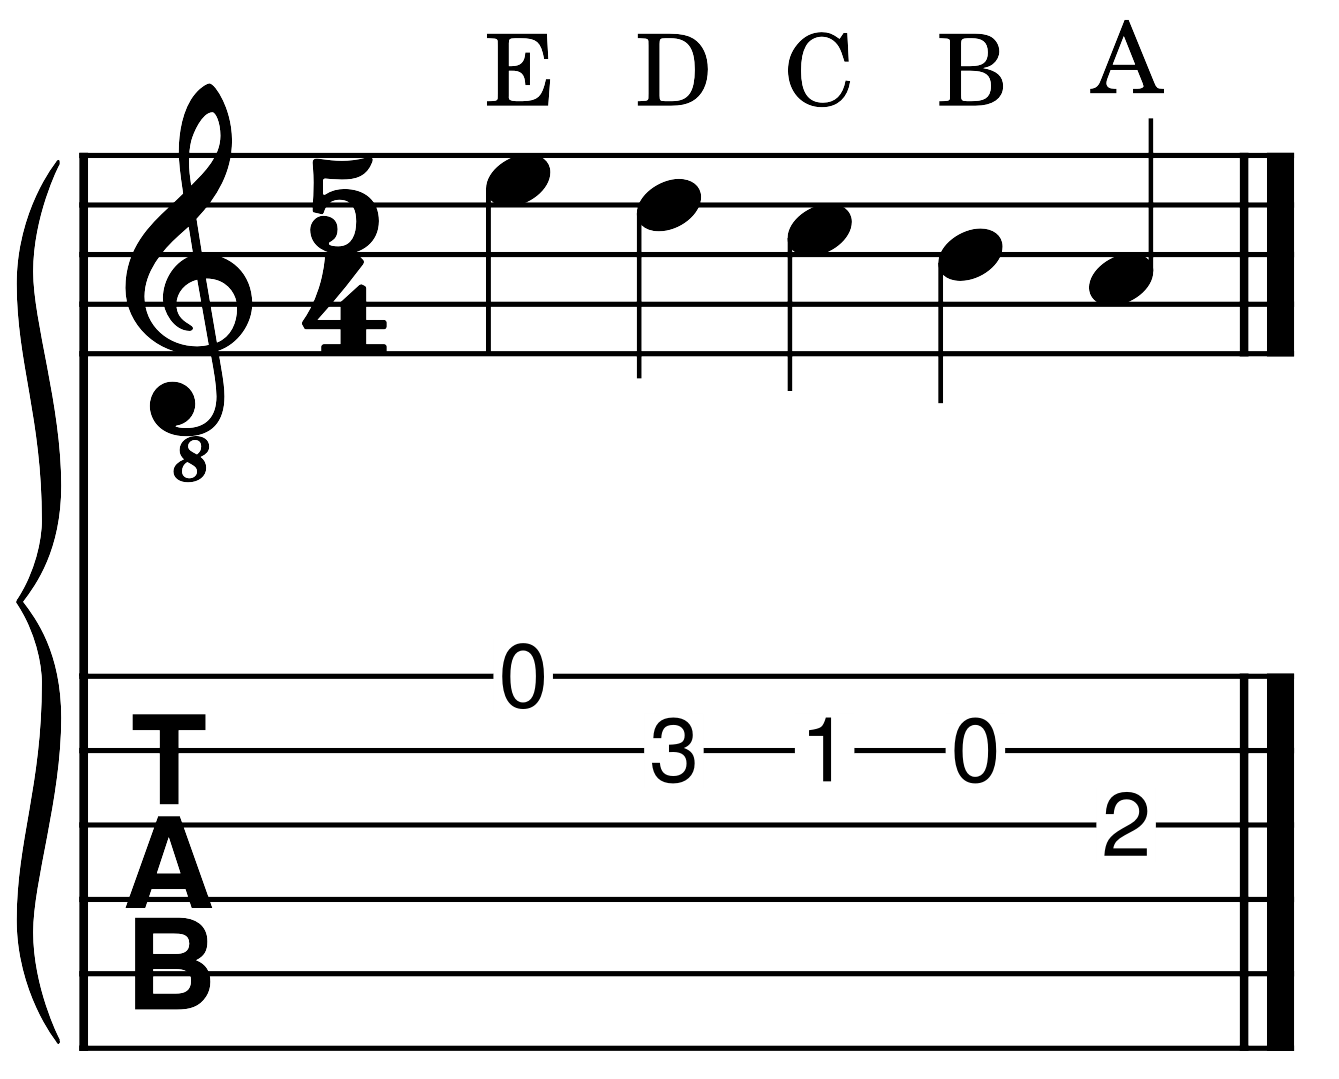
\includegraphics[height=0.12\textheight]{../../MuseScore/Guitar/NotesUsedInTetris_FirstPart.png}
	\caption{Notes used for the first part of the Tetris tune}
	\label{fig:notes_for_tetris_first_part}
\end{figure}

In \autoref{fig:tetris_simple_first_part} the first part of the Tetris tune is written. Note the dotted note in measure 3. The full tune requires to learn about sharps and flats. So we will play the full tune later.

\begin{figure}[h]
	\centering
	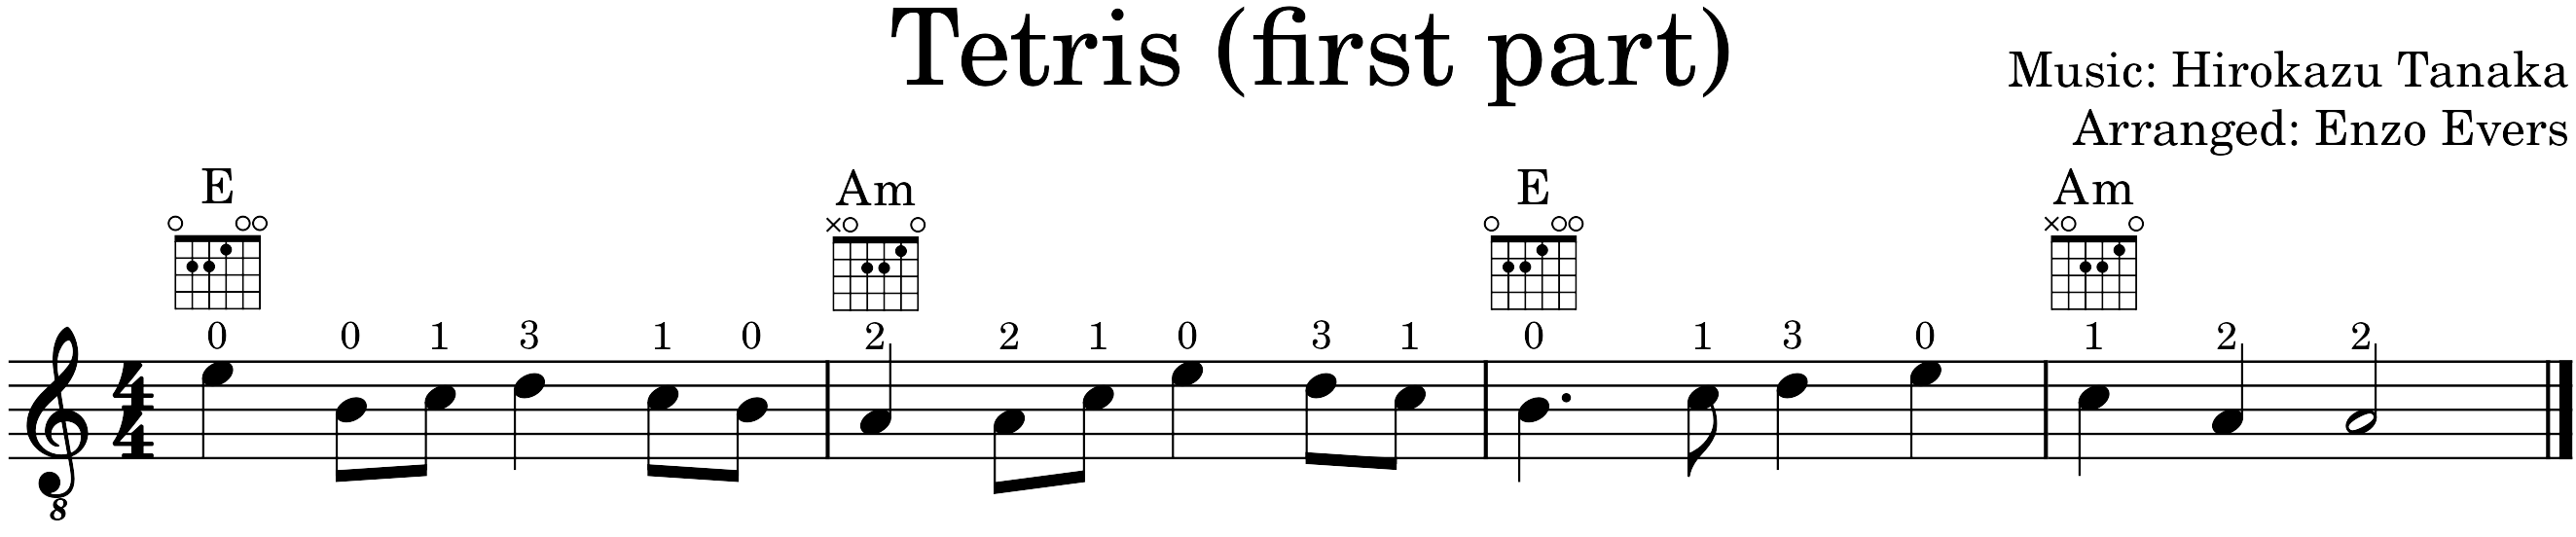
\includegraphics[width=\textwidth]{../../MuseScore/Guitar/GuitarTetrisFirstPart.png}
	\caption{First part of the Tetris tune}
	\label{fig:tetris_simple_first_part}
\end{figure}

\infobox{The "Tetris" tune is derived from a Russian folk song called "Korobeiniki", which is based the a similar named poem written by Nikolay Nekrasov. \cite{KorobeinikiWiki}}

\newpage

We have now played all non-sharp/flat notes. But each note can be placed in different positions, and with different pitches.

Let's take the melody of "Memory" from the musical "Cats" \autoref{fig:memory_cats}. It uses most of the notes we already learned, but also uses a lower G, F, and E (\autoref{fig:notes_g_f_e_3}).


\begin{figure}[h]
	\centering
	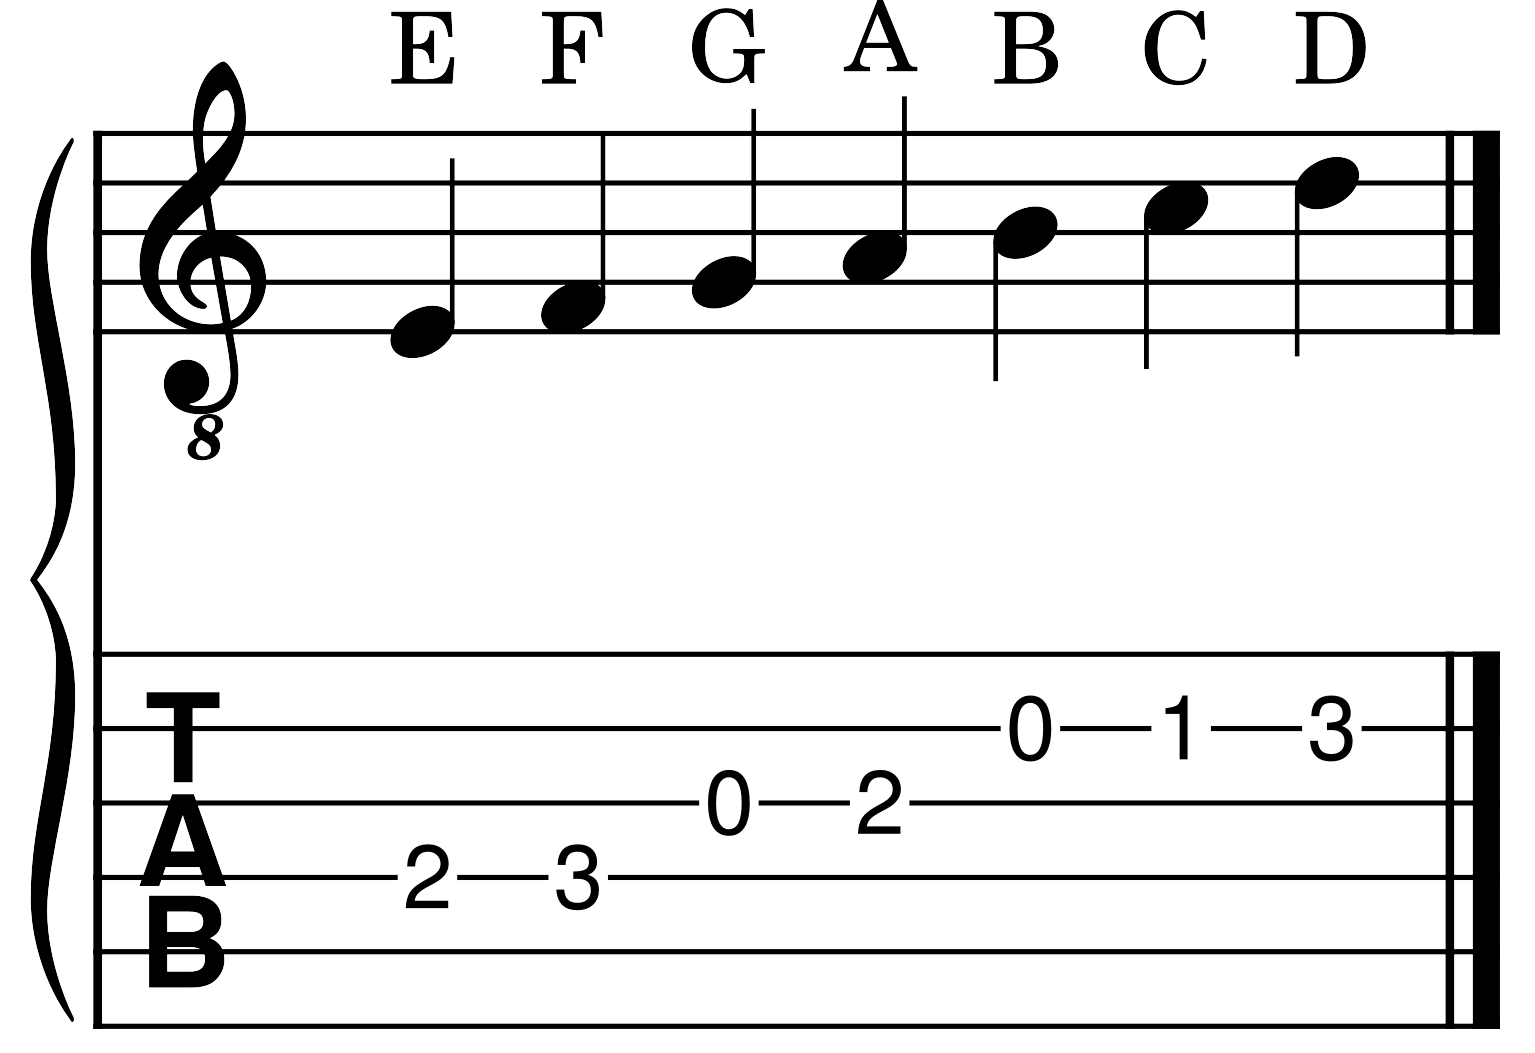
\includegraphics[height=0.12\textheight]{../../MuseScore/Guitar/NotesUsedInMemoryCats.png}
	\caption{The G, F, and G, notes on the 3rd and 4th strings}
	\label{fig:notes_g_f_e_3}
\end{figure}

It also uses a new symbol. The \textbf{tie} symbol (seen to connect notes from measure 5 and 6 in \autoref{fig:memory_cats}). This symbol indicates that the duration of the first note that starts the tie has the summed duration of all consecutive identical note. All identical notes after the note that starts the tie are therefore not played

\begin{figure}[h]
	\centering
	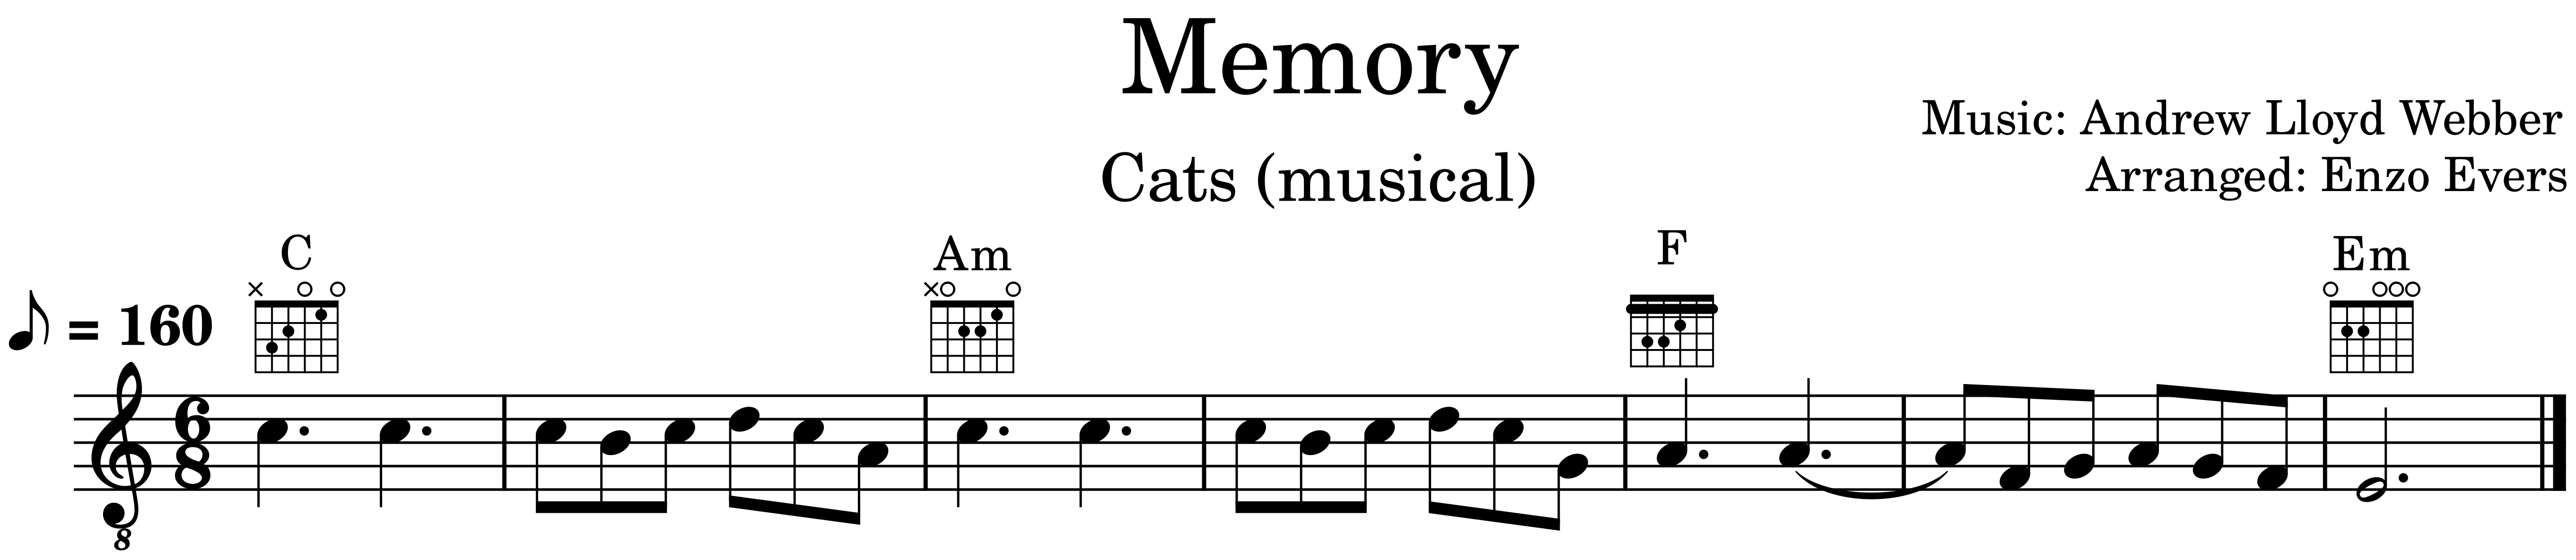
\includegraphics[width=\textwidth]{../../MuseScore/Guitar/GuitarMemoryCats.png}
	\caption{Memory from the musical Cats}
	\label{fig:memory_cats}
\end{figure}

Another song that you know that uses all the notes that you've learned so far is Happy birthday {\autoref{fig:happy_birthday}}. 

\begin{figure}[h]
	\centering
	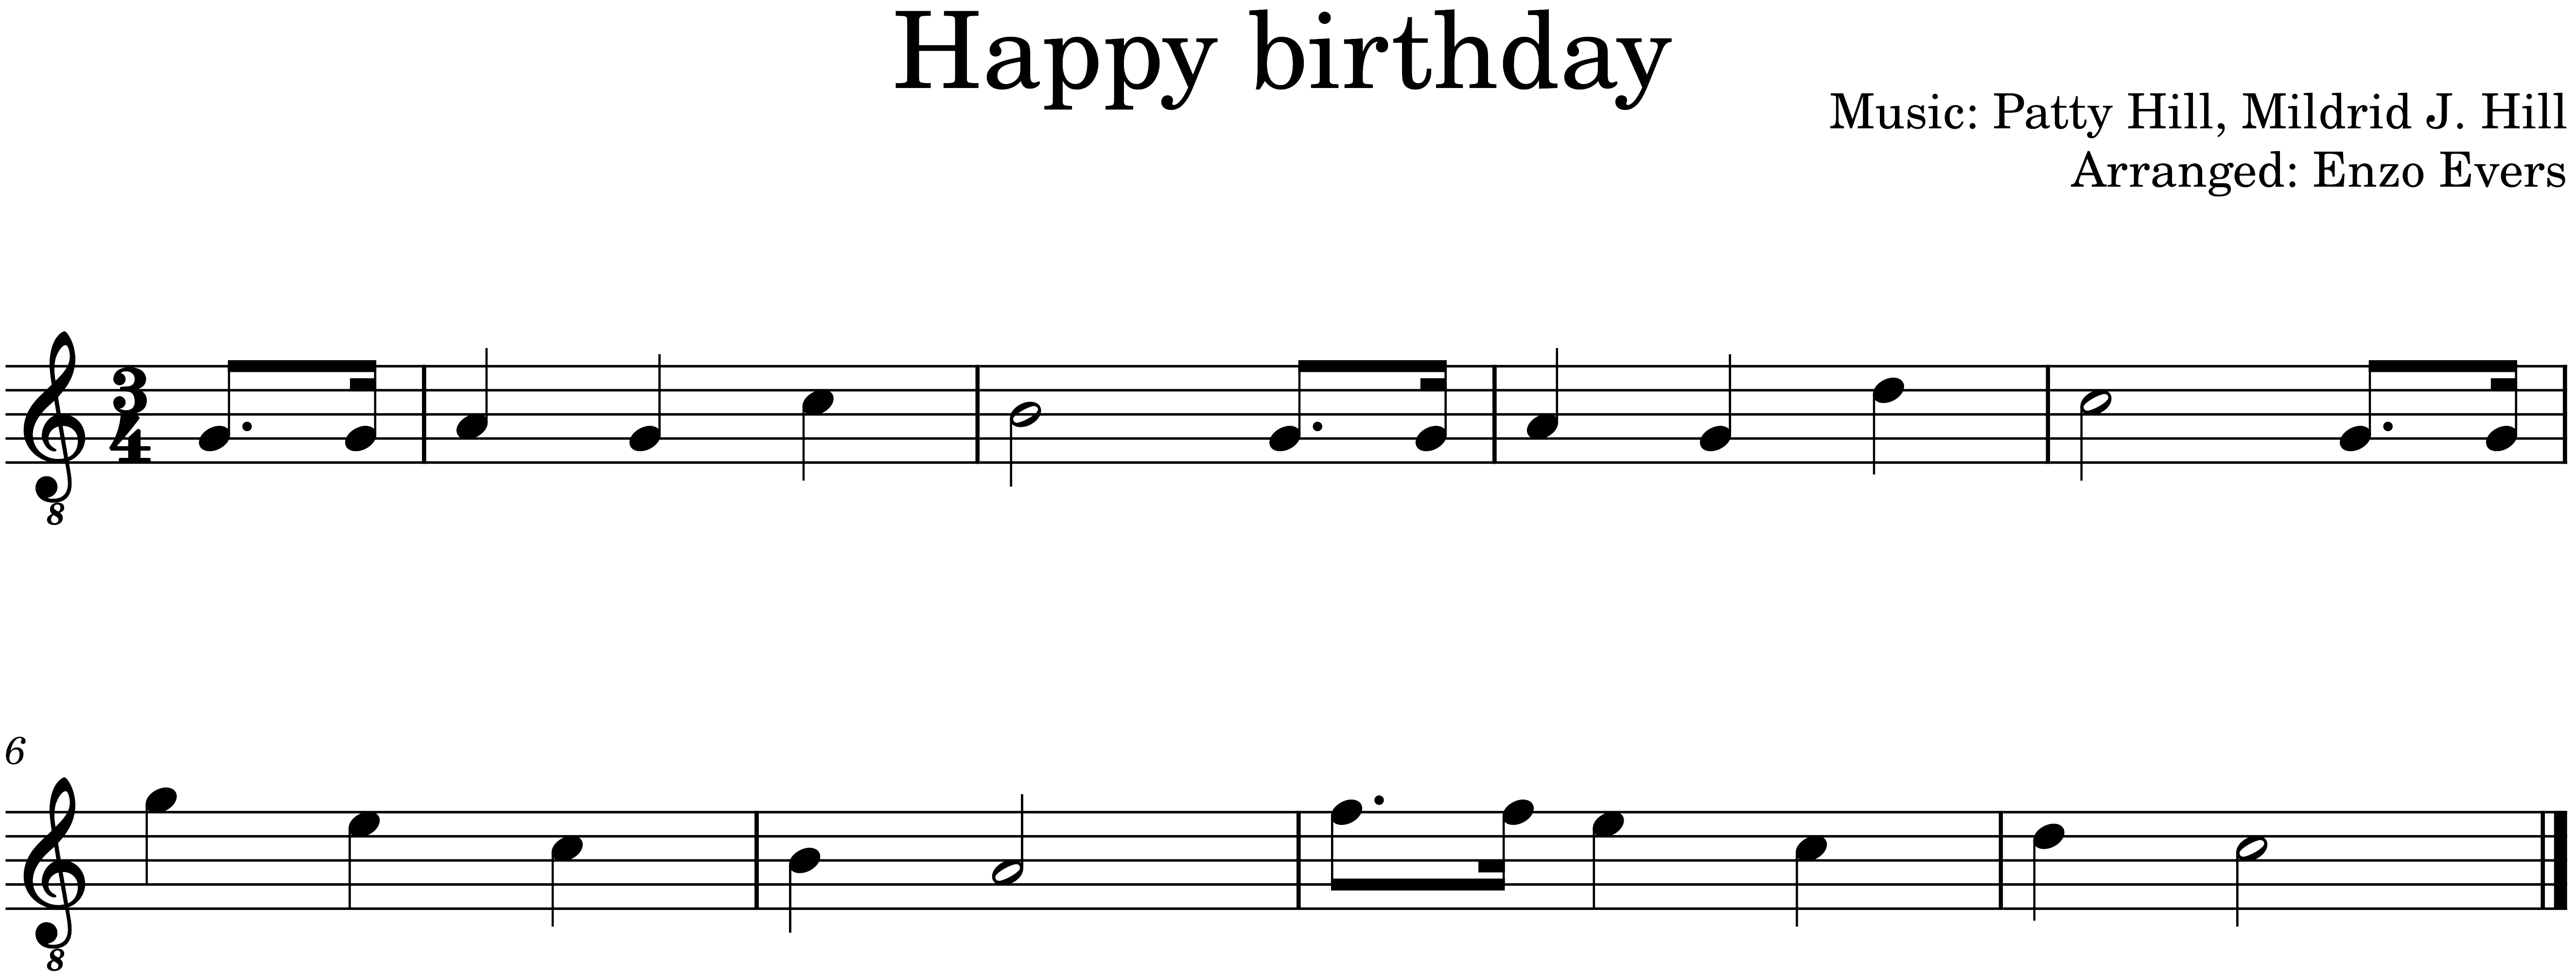
\includegraphics[width=\textwidth]{../../MuseScore/Guitar/GuitarHappyBirthday.png}
	\caption{Happy birthday}
	\label{fig:happy_birthday}
\end{figure}

\newpage

In the following song you will learn the low C and D notes.

\begin{figure}[h]
	\centering
	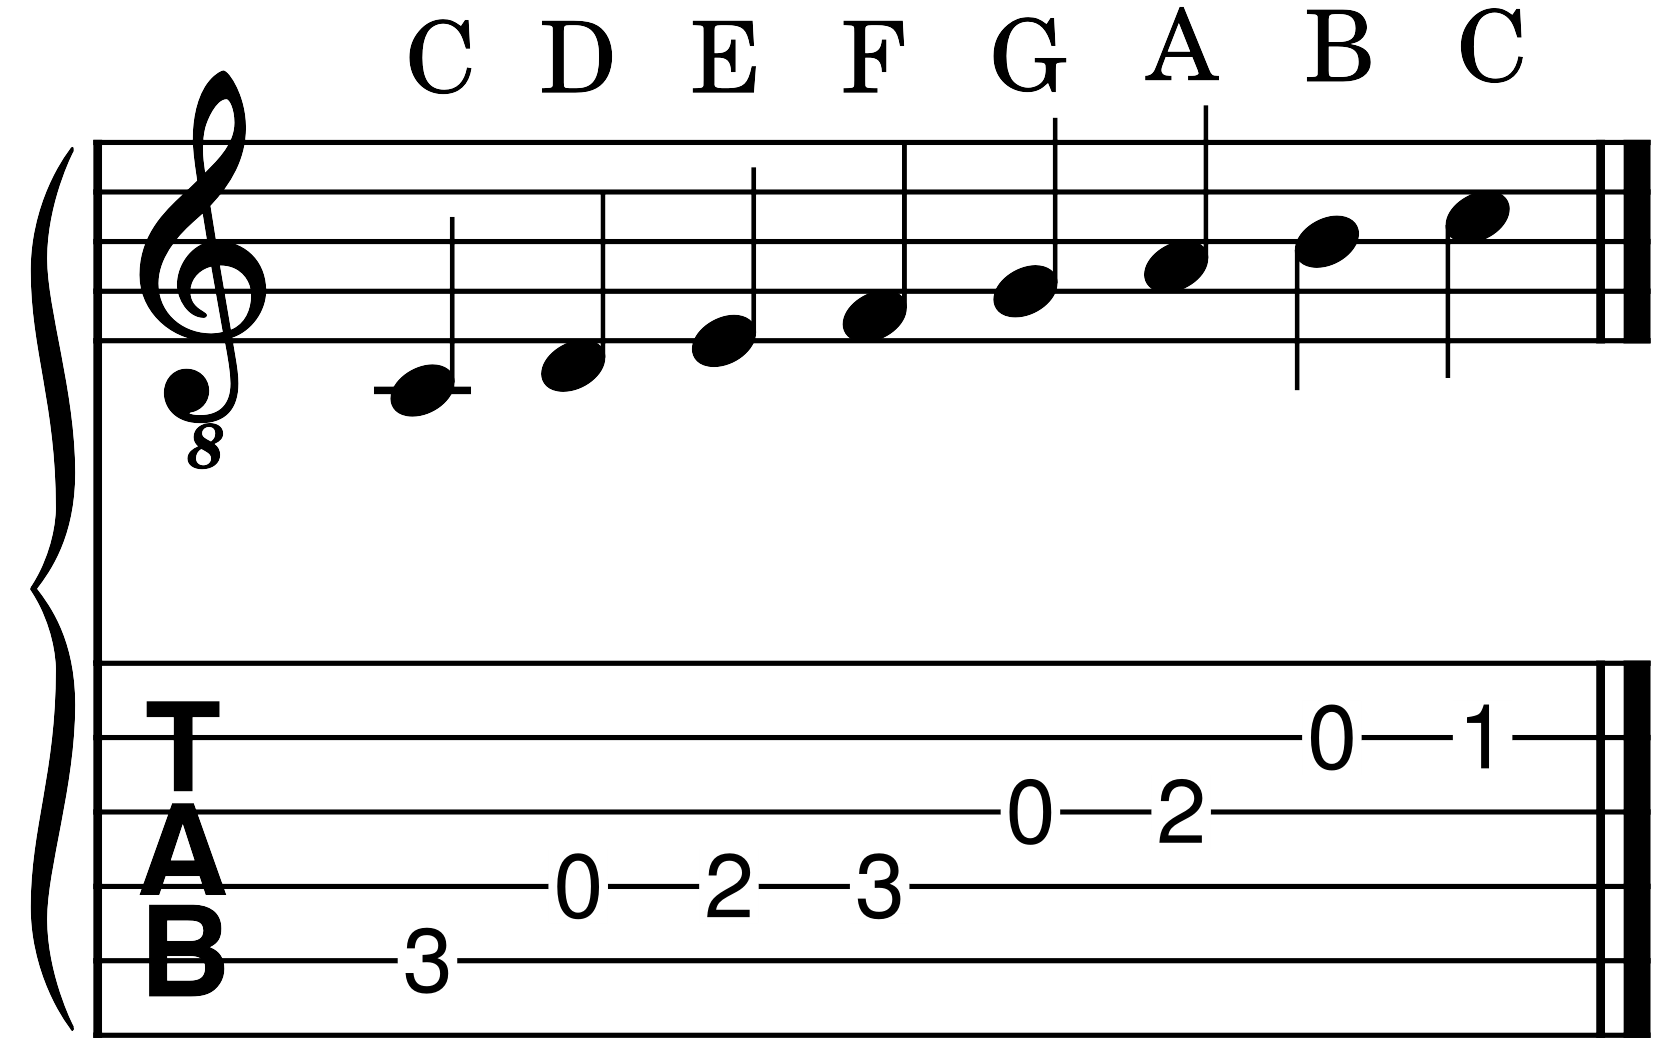
\includegraphics[height=0.12\textheight]{../../MuseScore/Guitar/GuitarNotesUsedInVogeltjesdans.png}
	\caption{Notes used for the song "De Vogeltjesdans"}
	\label{fig:guitar_notes_for_vogeltjesdans}
\end{figure}

\infobox{In \autoref{fig:guitar_notes_for_vogeltjesdans} you not only see the notes used in the song, but you also see the C major scale. Later on we will talk more about scales.}

\begin{figure}[h]
	\centering
	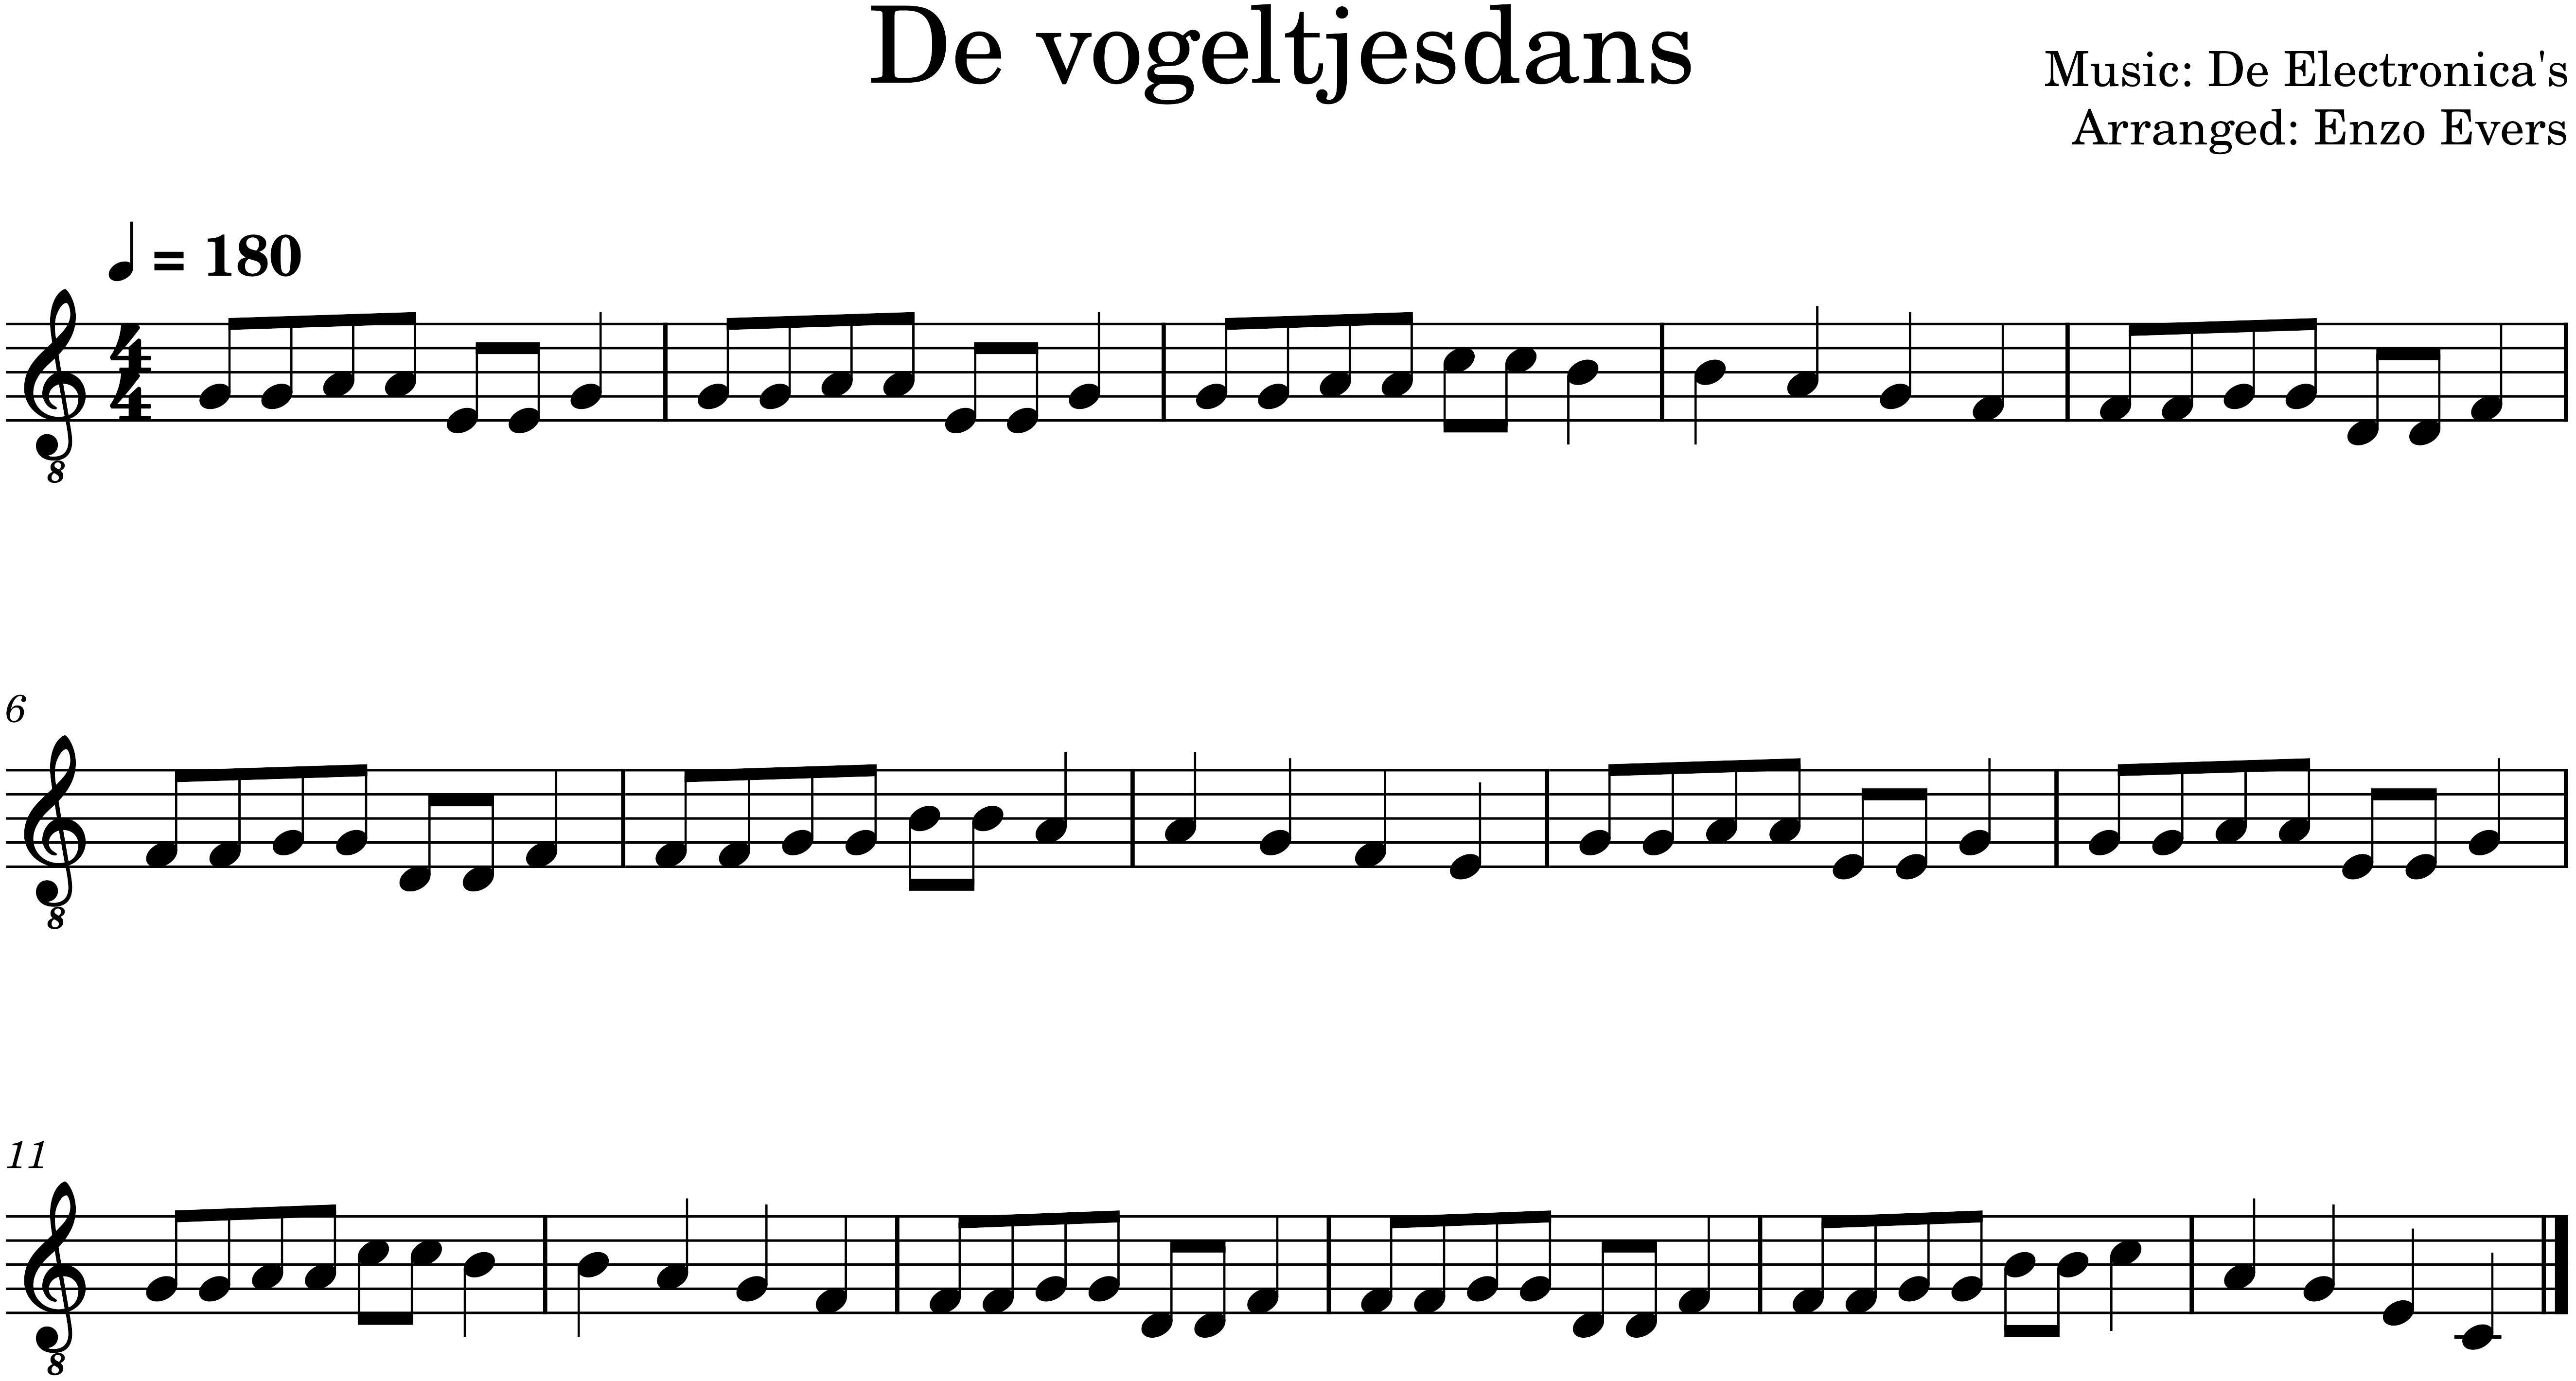
\includegraphics[width=\textwidth]{../../MuseScore/Guitar/GuitarVogeltjesdansDeElectronicas.png}
	\caption{De vogeltjesdans - De Electronica's}
	\label{fig:guitar_vogeltjesdans}
\end{figure}

\infobox{While most people know this as the Dutch titled "De vogeltjesdans". It is based on the original song called "Der Ententanz" composed by Werner Thomas. \cite{DeVogeltjesDansWiki}}

\newpage

In the next song the low B, A, G, and E notes is introduced.

\begin{figure}[h]
	\centering
	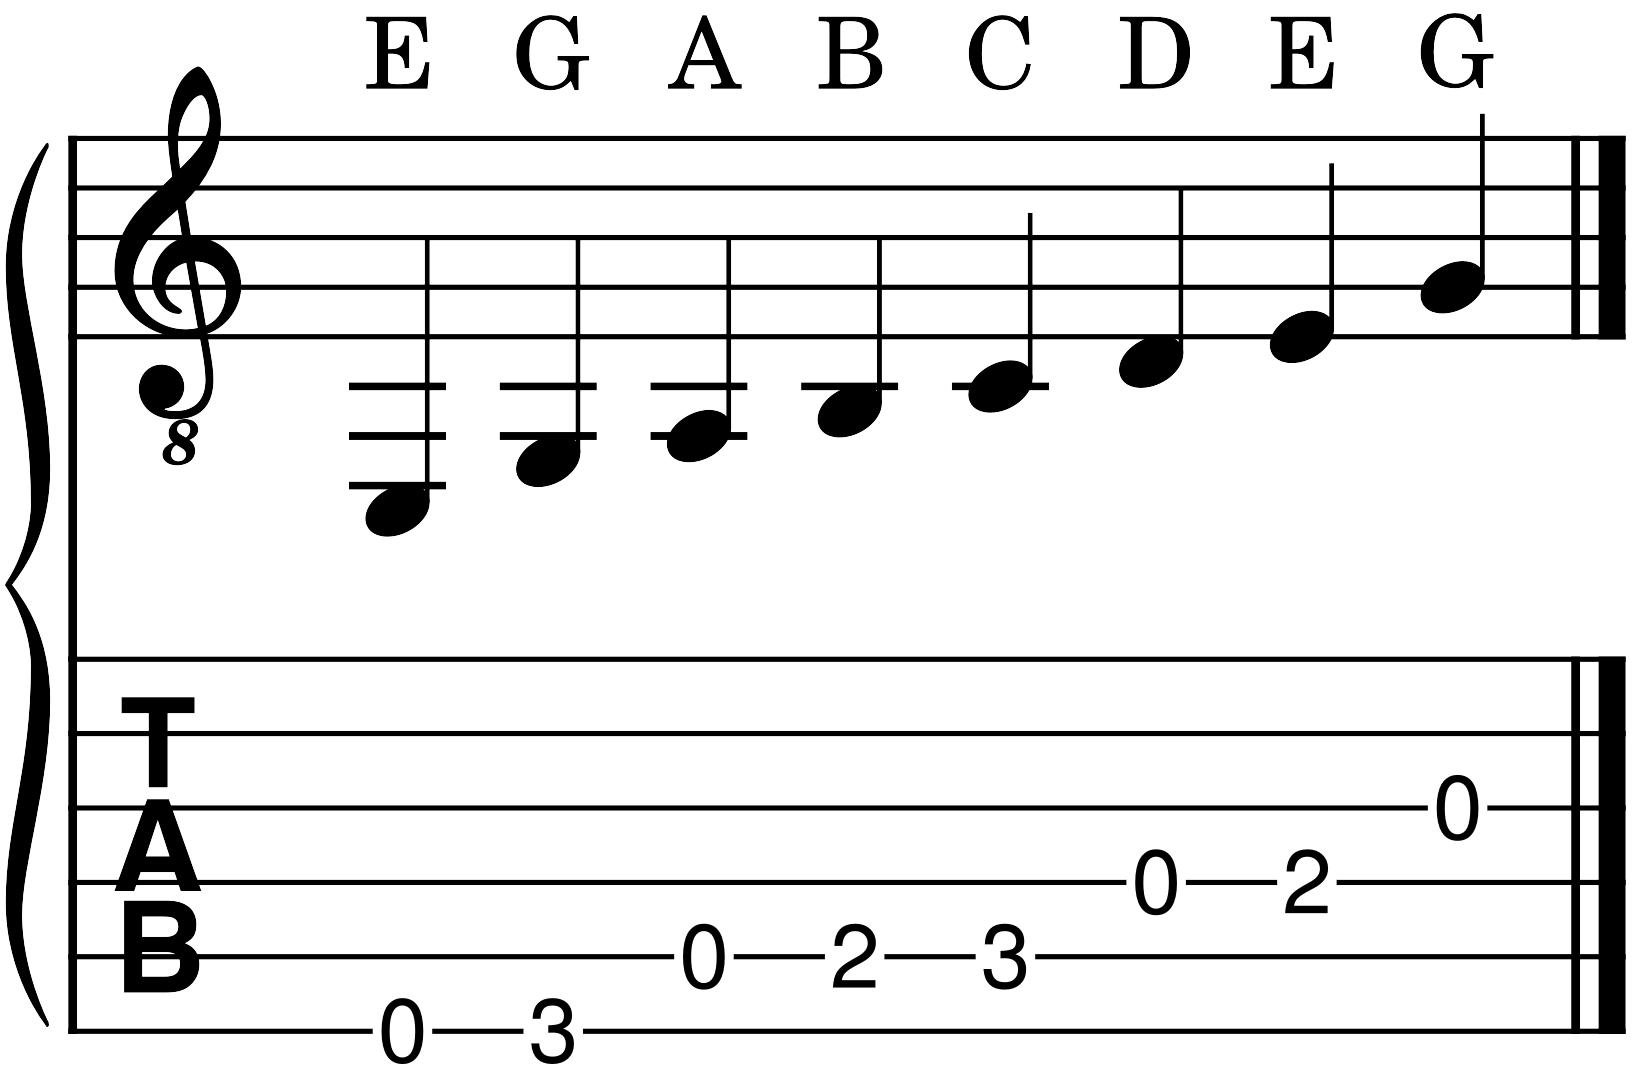
\includegraphics[height=0.12\textheight]{../../MuseScore/Guitar/GuitarNotesUsedInSevenNationArmy.png}
	\caption{Notes used for the song "Seven Nation Army"}
	\label{fig:guitar_notes_for_seven_nation_army}
\end{figure}

Before playing \autoref{fig:guitar_seven_nation_army}. Lets see how these notes work that are below the normal lines. In the beginning of this chapter, the names of the notes that correspond to the lines of the staff where shown (\autoref{fig:music_note_names_on_staff}). Note there that each line and space between the lines had the sequence of "A, B, C, D, E, F, G, A, B, etc." if you go up up on the staff lines (and the other direction if you go on the staff lines). This sequence simply continues below and above the normal staff lines.

\begin{figure}[h]
	\centering
	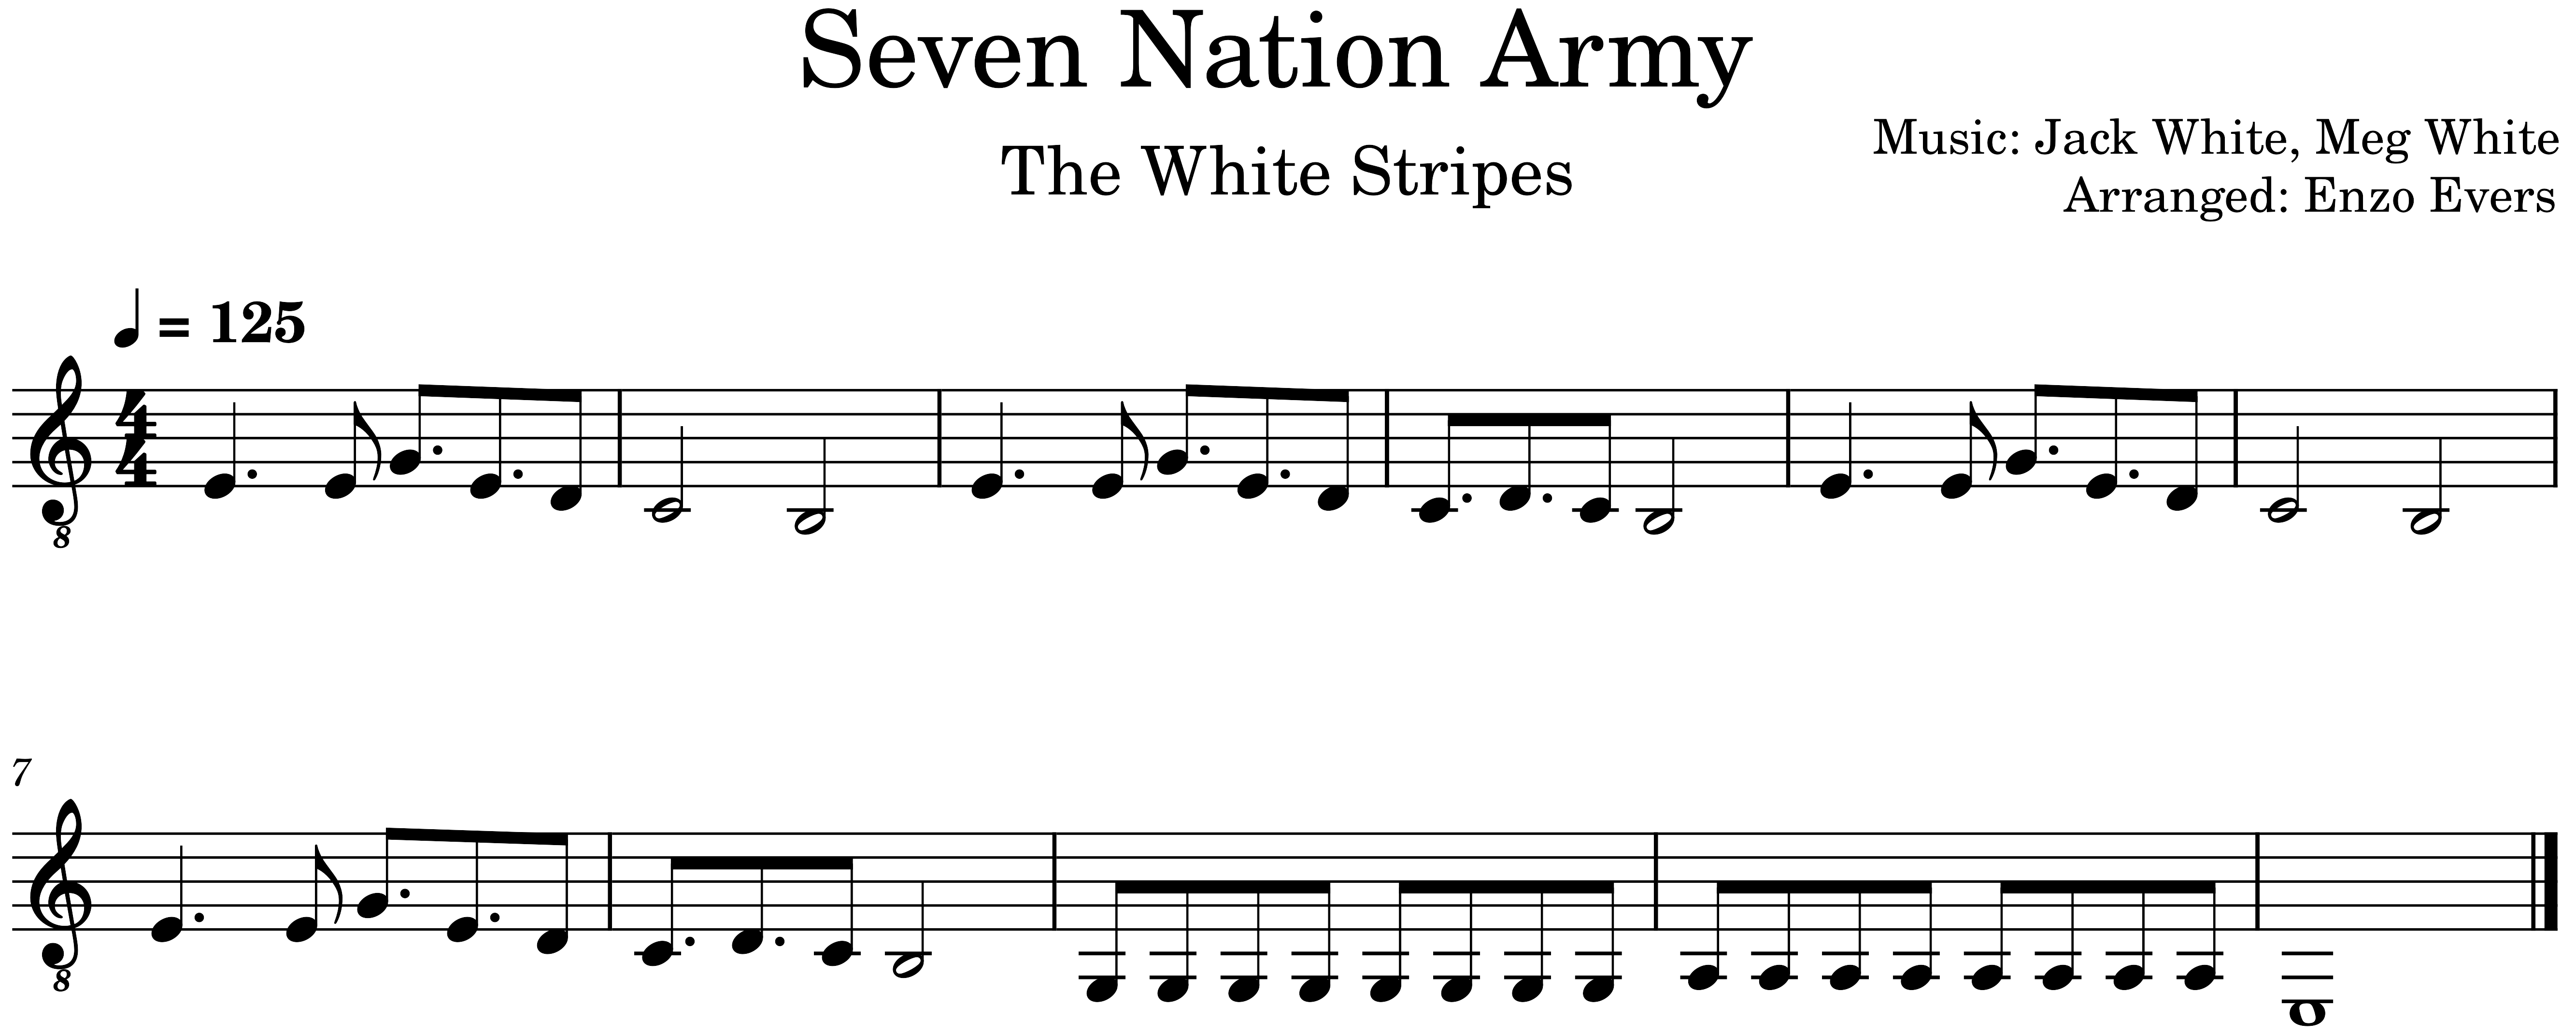
\includegraphics[width=\textwidth]{../../MuseScore/Guitar/GuitarSevenNationArmyTheWhiteStripes.png}
	\caption{Seven Nation Army - The White Stripes}
	\label{fig:guitar_seven_nation_army}
\end{figure}

\newpage

To introduce the last non-sharp/flat note withing the first 3 frets, we will play the first part from "Californication" from "Red Hot Chili Peppers". This introduces the low F note.

\begin{figure}[h]
	\centering
	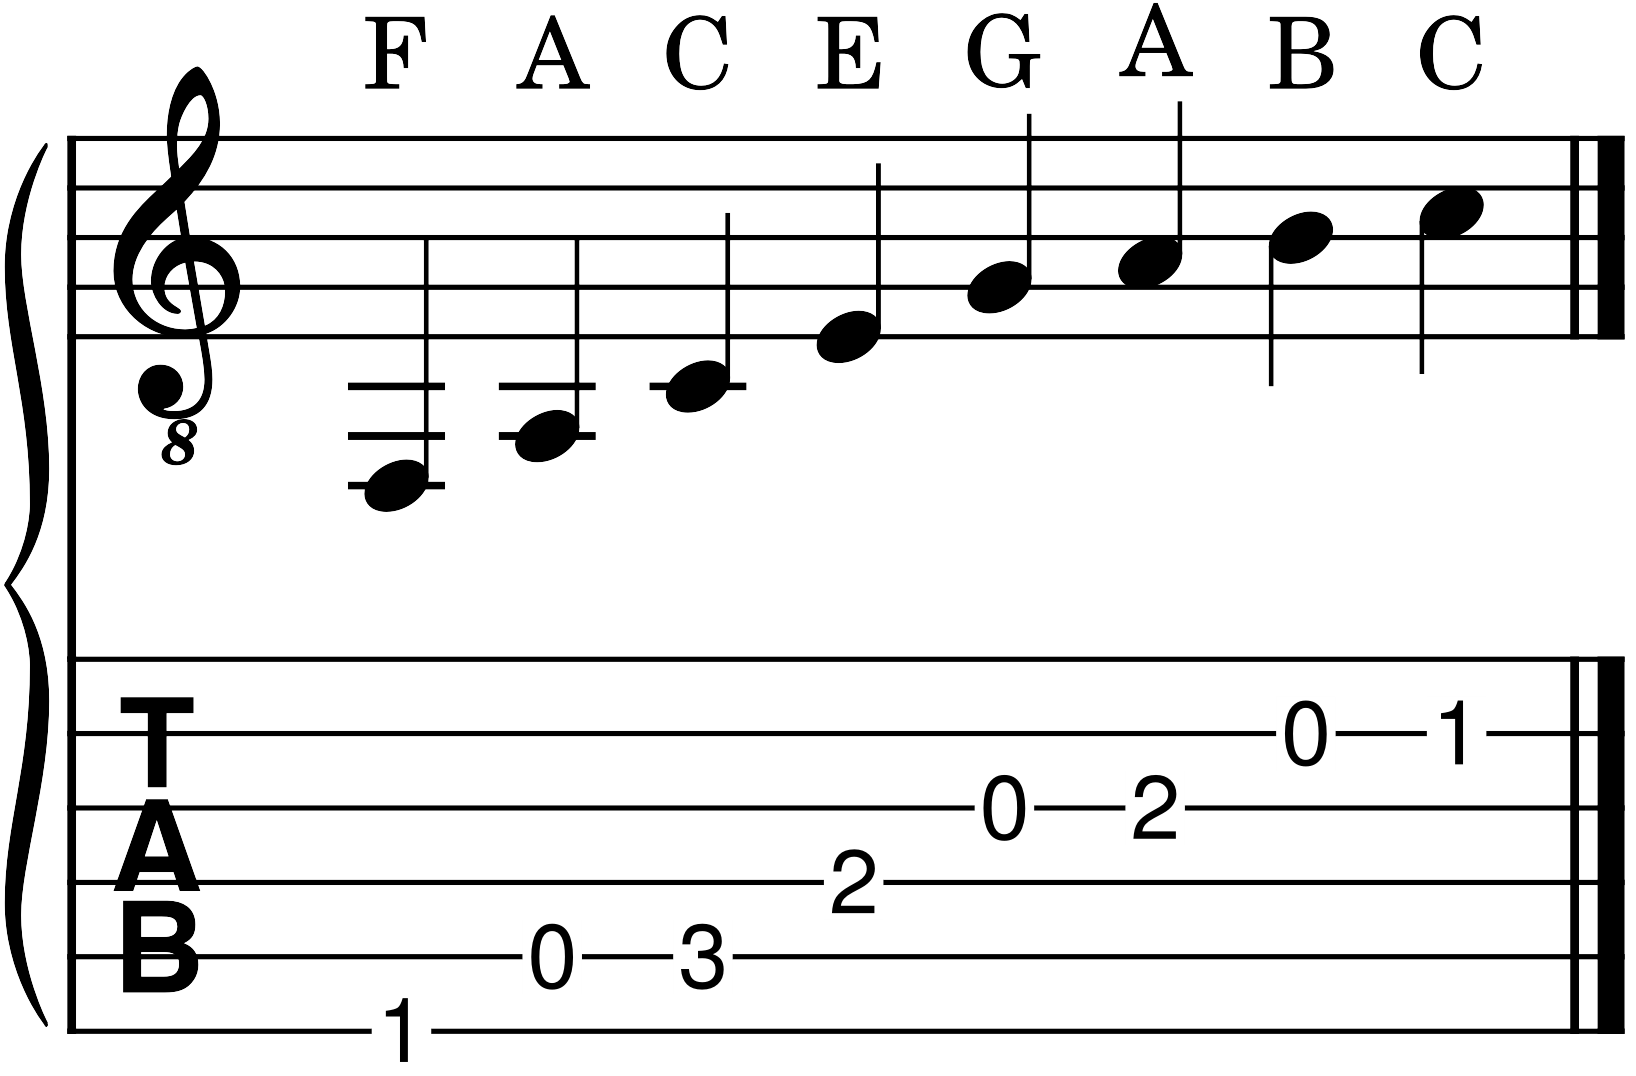
\includegraphics[height=0.12\textheight]{../../MuseScore/Guitar/GuitarNotesUsedInCalifornication.png}
	\caption{Notes used for the song "Californication"}
	\label{fig:guitar_notes_for_californication}
\end{figure}

Note the fingering in \autoref{fig:guitar_californication}. In this piece, keep you fingers on the frets for the duration of the measure after playing them to let them ring.

\begin{figure}[h]
	\centering
	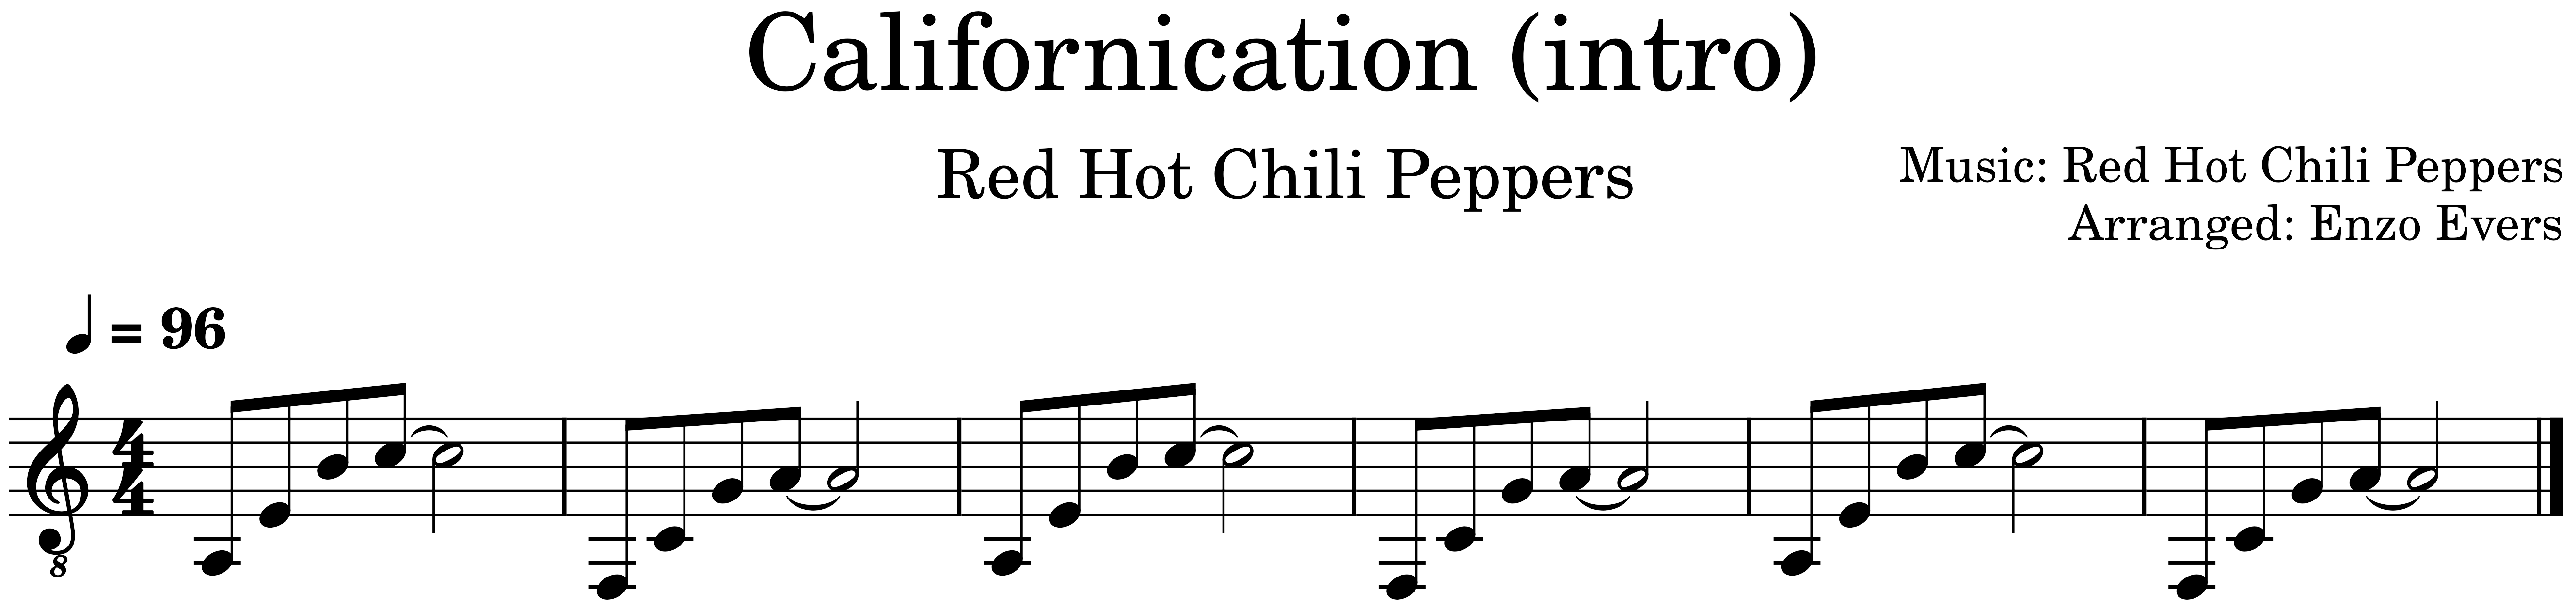
\includegraphics[width=\textwidth]{../../MuseScore/Guitar/GuitarCalifornicationRedHotChiliPeppers.png}
	\caption{Californication - Red Hot Chili Peppers}
	\label{fig:guitar_californication}
\end{figure}

\newpage

\section{Sharps and flats}

In the beginning of this method it was already mentioned that sharps $\sharp$ increase the note by a half step and flats $\flat$ decrease the note by a half step. It has also been mentioned that sharps and flats are valid for the duration of a measure. If a note should get its 'normal' sound back, a natural $\natural$ symbol is placed in front of it. This undoes the sharp/flat for the rest of the measure (until another sharp/flat is placed).

What has not been mentioned yet, is that a sharp/flat placed at a note is valid only for that pitch of the note (position on the sheet music). See for example \autoref{fig:guitar_usage_of_sharps_and_naturals}. Here you see that the first G (open third string) got a sharp, and is therefore now played a half tone (1 fret) higher on the 1st fret. The G that is played one octave higher on the first string is still a G. When the G note then gets a natural sign, it becomes the normal G note again which is played on the open third string. The same example can be given for flats (\autoref{fig:guitar_usage_of_flats_and_naturals}).

\begin{figure}[h]
	\begin{subfigure}[b]{0.45\textwidth}
		\centering
		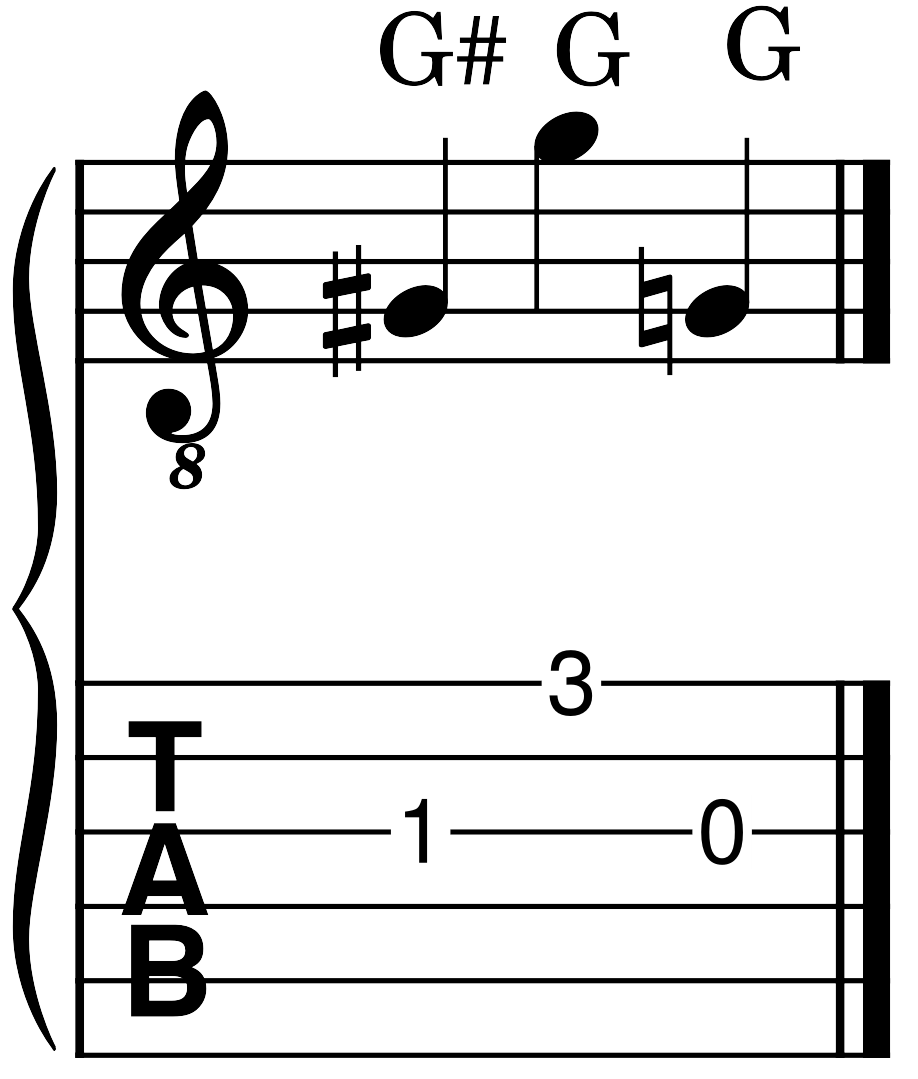
\includegraphics[height=0.15\textheight]{../../MuseScore/Guitar/GuitarSharpApplyExample.png}
		\caption{Usage of sharps and naturals}
		\label{fig:guitar_usage_of_sharps_and_naturals}
	\end{subfigure}
	\hfill
	\begin{subfigure}[b]{0.45\textwidth}
		\centering
		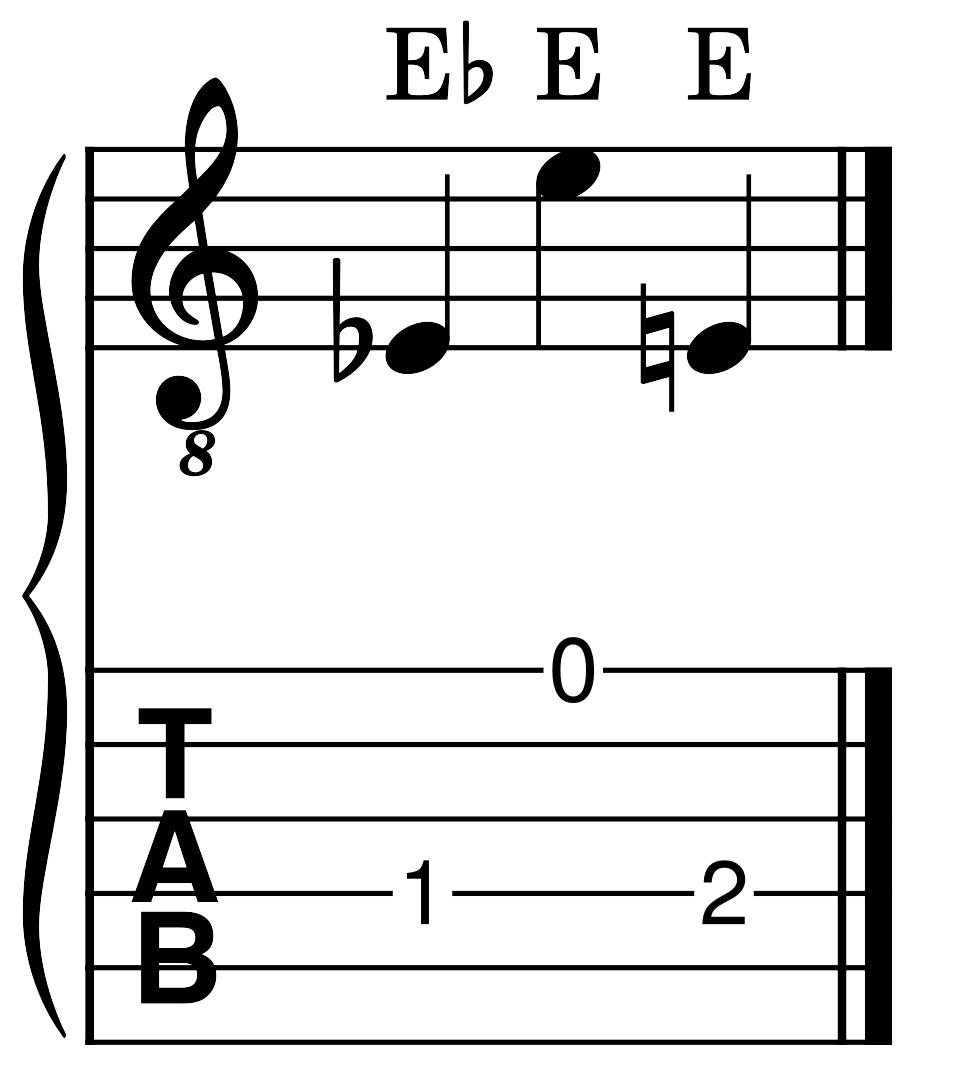
\includegraphics[height=0.15\textheight]{../../MuseScore/Guitar/GuitarFlatApplyExample.png}
		\caption{Usage of flats and naturals}
		\label{fig:guitar_usage_of_flats_and_naturals}
	\end{subfigure}
	\caption{Sharps, flats and naturals}
\end{figure}

Sometimes a song uses a note with a flat or sharp a lot of times. It can then be considered to be in a certain key (we will come back to that later). It is then not desired to add sharps/flats all over the sheet music. That could get messy. Instead, the sharps/flats used for the song are shown as the beginning of the piece and apply to all pitches of the notes (unless natural symbols are used). Note that this is different than adding sharps inside a measure, there it only applied to that specific pitch.

See for example \autoref{fig:guitar_sharps_at_start_of_music} and \autoref{fig:guitar_flats_at_start_of_music}.

\begin{figure}[h]
	\centering
	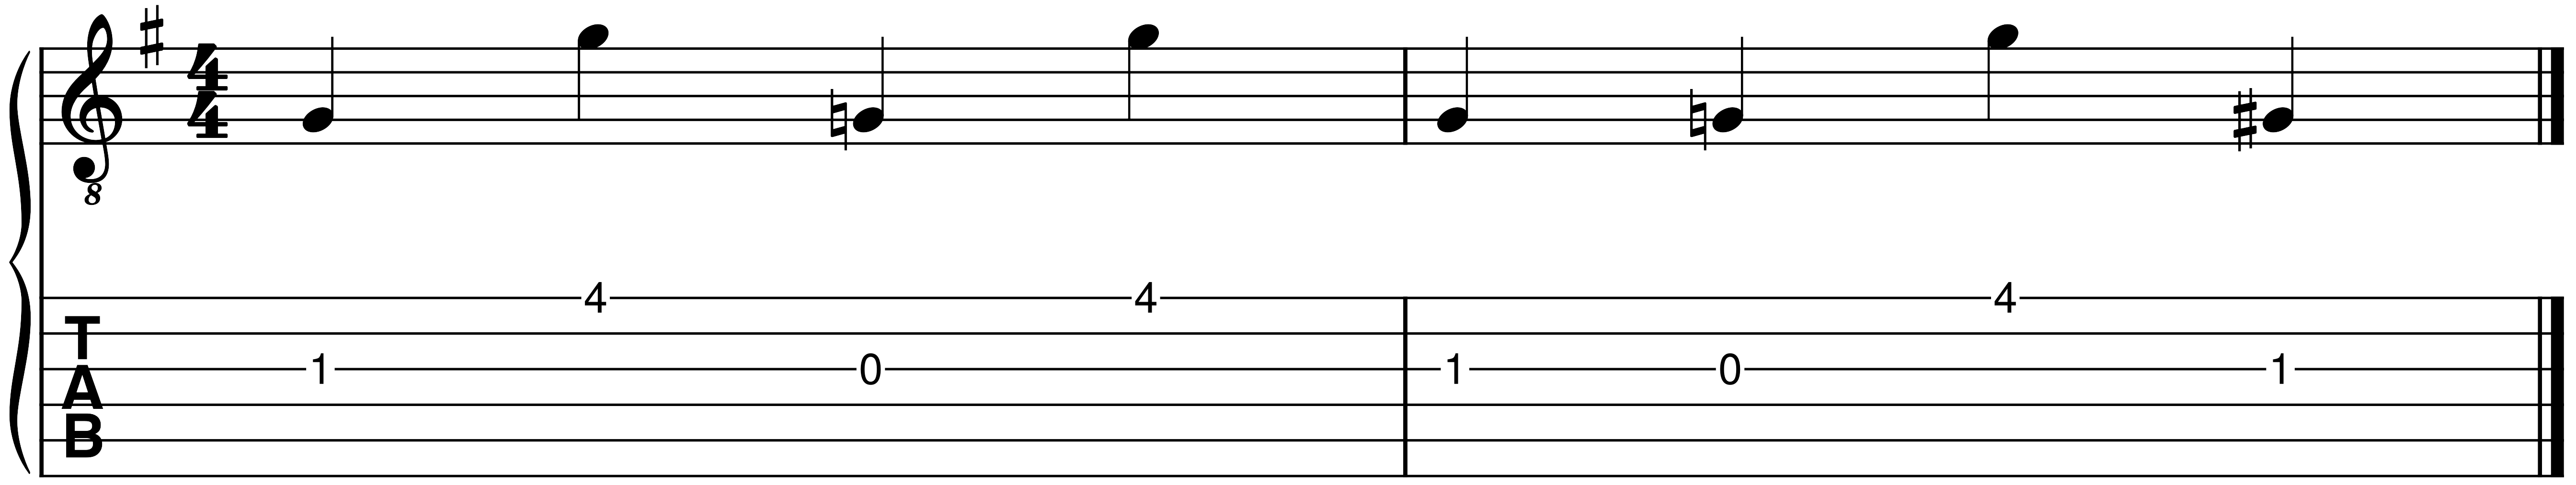
\includegraphics[width=\textwidth]{../../MuseScore/Guitar/GuitarKeySharpExample.png}
	\caption{Example of adding sharps at the beginning of the music}
	\label{fig:guitar_sharps_at_start_of_music}
\end{figure}

\begin{figure}[h]
	\centering
	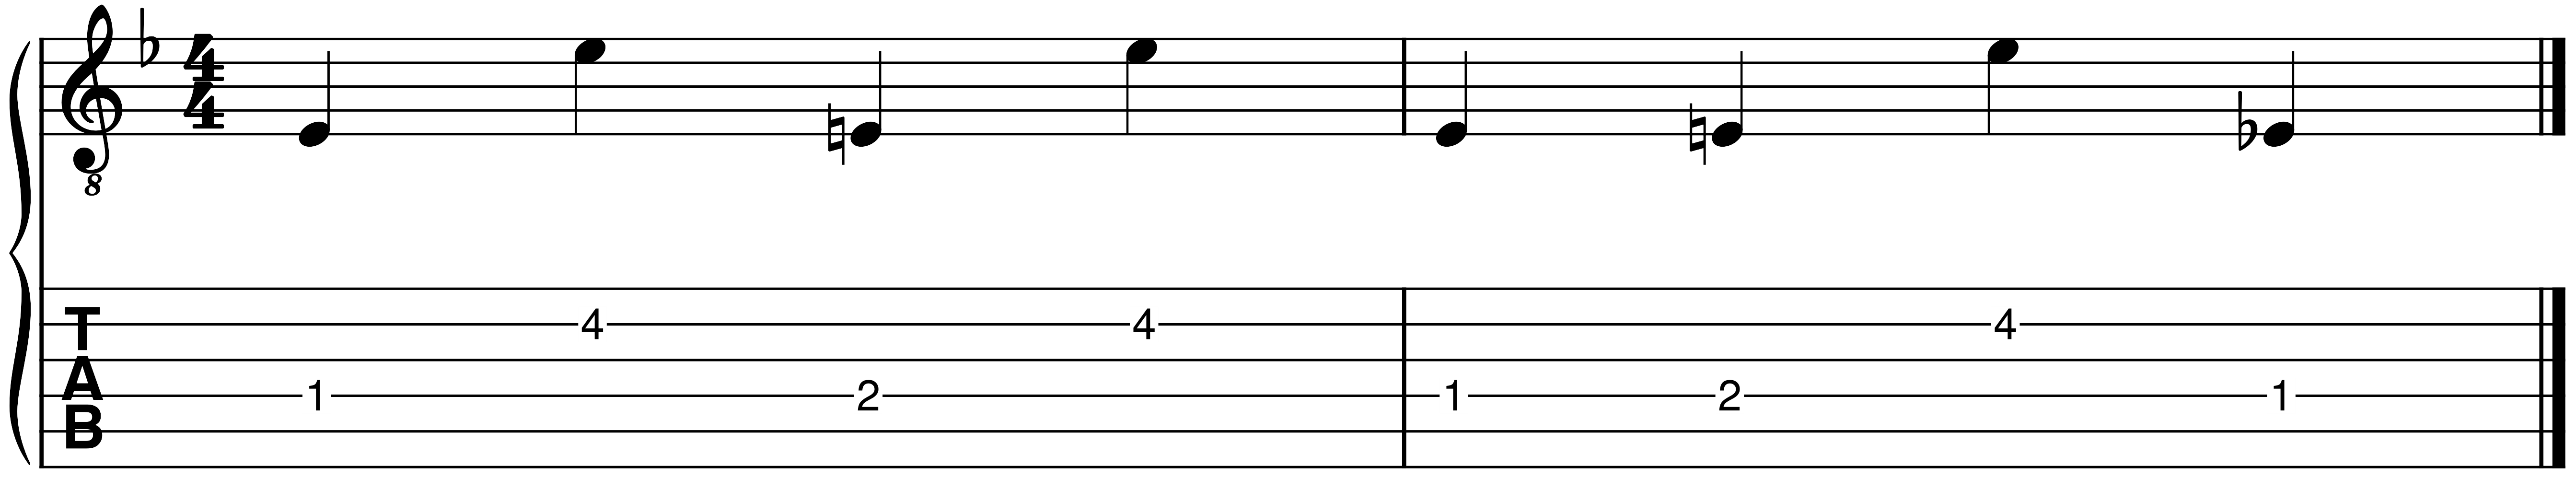
\includegraphics[width=\textwidth]{../../MuseScore/Guitar/GuitarKeyFlatExample.png}
	\caption{Example of adding flats at the beginning of the music}
	\label{fig:guitar_flats_at_start_of_music}
\end{figure}

\newpage

Before playing some pieces to learn the sharps and flats, lets first show the sharps and flats on the fretboard again:

\begin{figure}[h]
	\centering
	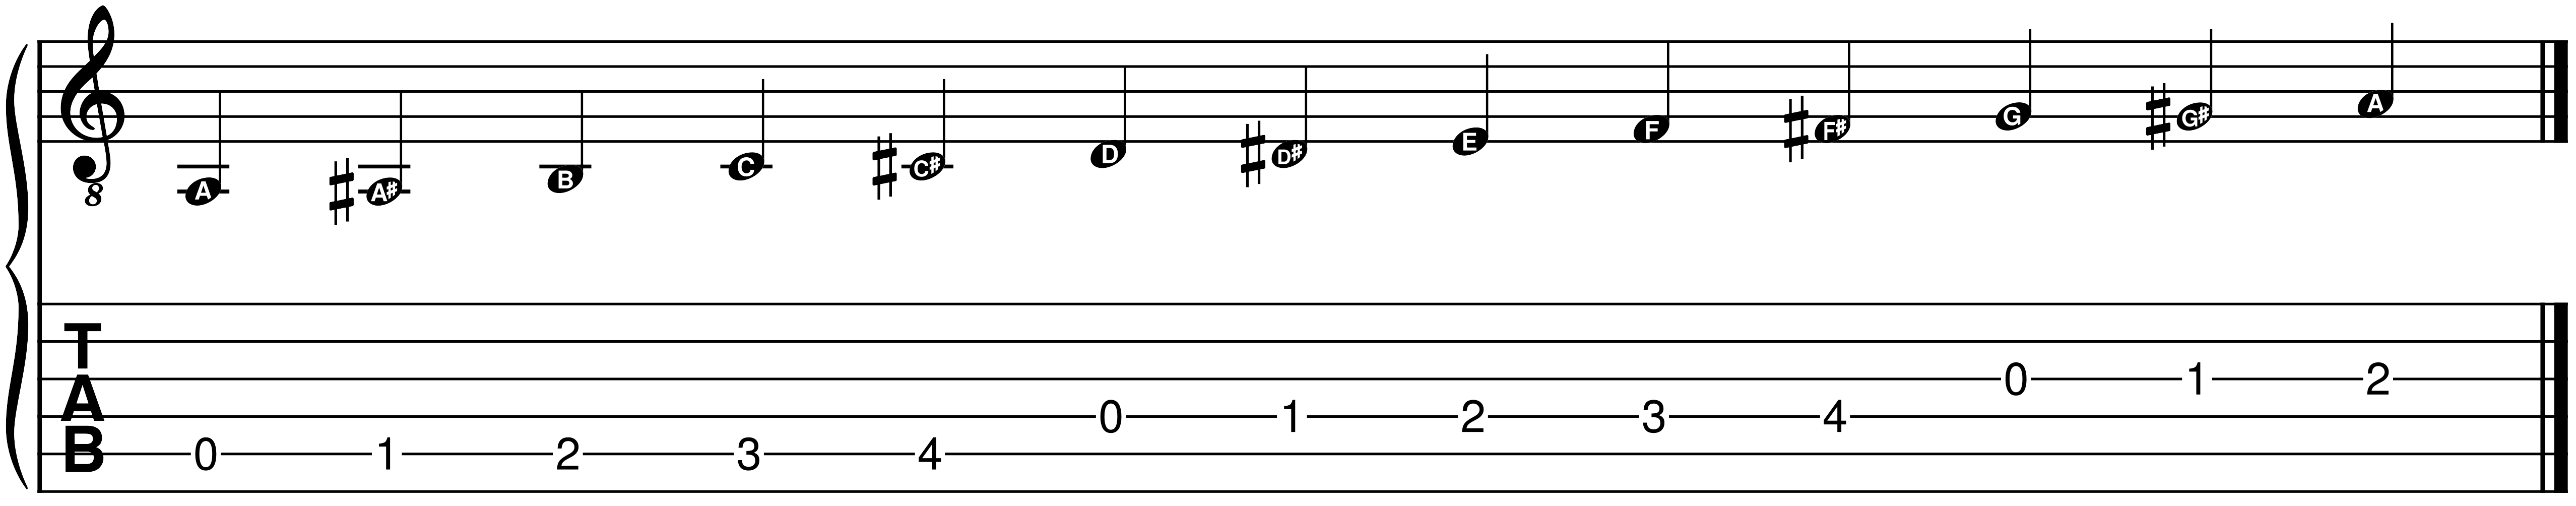
\includegraphics[width=\textwidth]{../../MuseScore/Guitar/PitchesSharpsMultiString.png}
	\caption{An octave from A to A on the multiple strings using sharps}
	\label{fig:guitar_string_a_octave_multi_string_sharps_chap_music_notation}
\end{figure}

\begin{figure}[h]
	\centering
	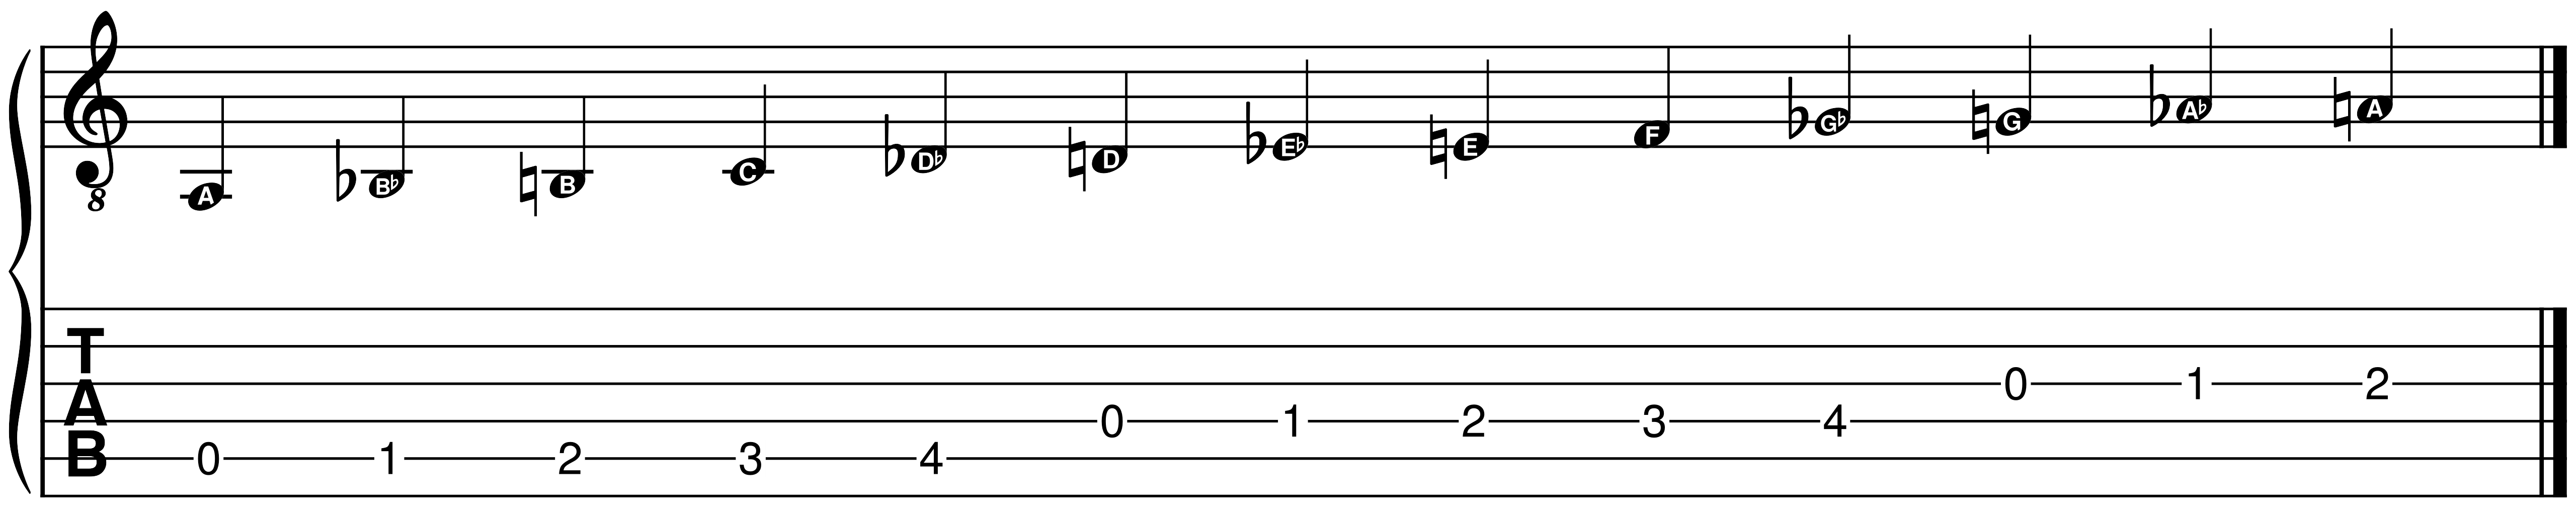
\includegraphics[width=\textwidth]{../../MuseScore/Guitar/PitchesFlatsMultiString.png}
	\caption{An octave from A to A on the multiple strings using flats and naturals}
	\label{fig:guitar_string_a_octave_multi_string_flats_chap_music_notation}
\end{figure}

Also remember that between each note, except for B-C and E-F, there is are two half steps. Between B-C and E-F there is only one half step.

\begin{table}[h]
	\centering
	\begin{tabular}{*{12}{P{5mm}}}
		\large{A} & \large{A\sharp} & \large{B} & \large{C} & \large{C\sharp} & \large{D} & \large{D\sharp} & \large{E} & \large{F} & \large{F\sharp} & \large{G} & \large{G\sharp} \\ \\
		\large{A} & \large{B\flat} & \large{B} & \large{C} & \large{D\flat} & \large{D} & \large{E\flat} & \large{E} & \large{F} & \large{G$\flat$}& \large{G} & \large{A\flat}
	\end{tabular}
	\caption{Sharp and flat intervals}
	\label{tab:guitar_sharp_flat_intervals}
\end{table}

Remember that a sharp and flat simply move the note a half step up or down respectively. So what would happen when the E note gets a $\sharp$? It would become an F. And what does an F$\flat$ resolve to? An E indeed. The same holds for the B-C interval. B$\sharp$ is the same as a C and a C$\flat$ is the same as a B.

\newpage

Previously we have already played Happy Birtday without any sharps or flats. But the music can be 'transposed' to a different key. This can introduce sharps/flats. Also in \autoref{fig:guitar_happy_birthday_sharps}.

\begin{figure}[h]
	\centering
	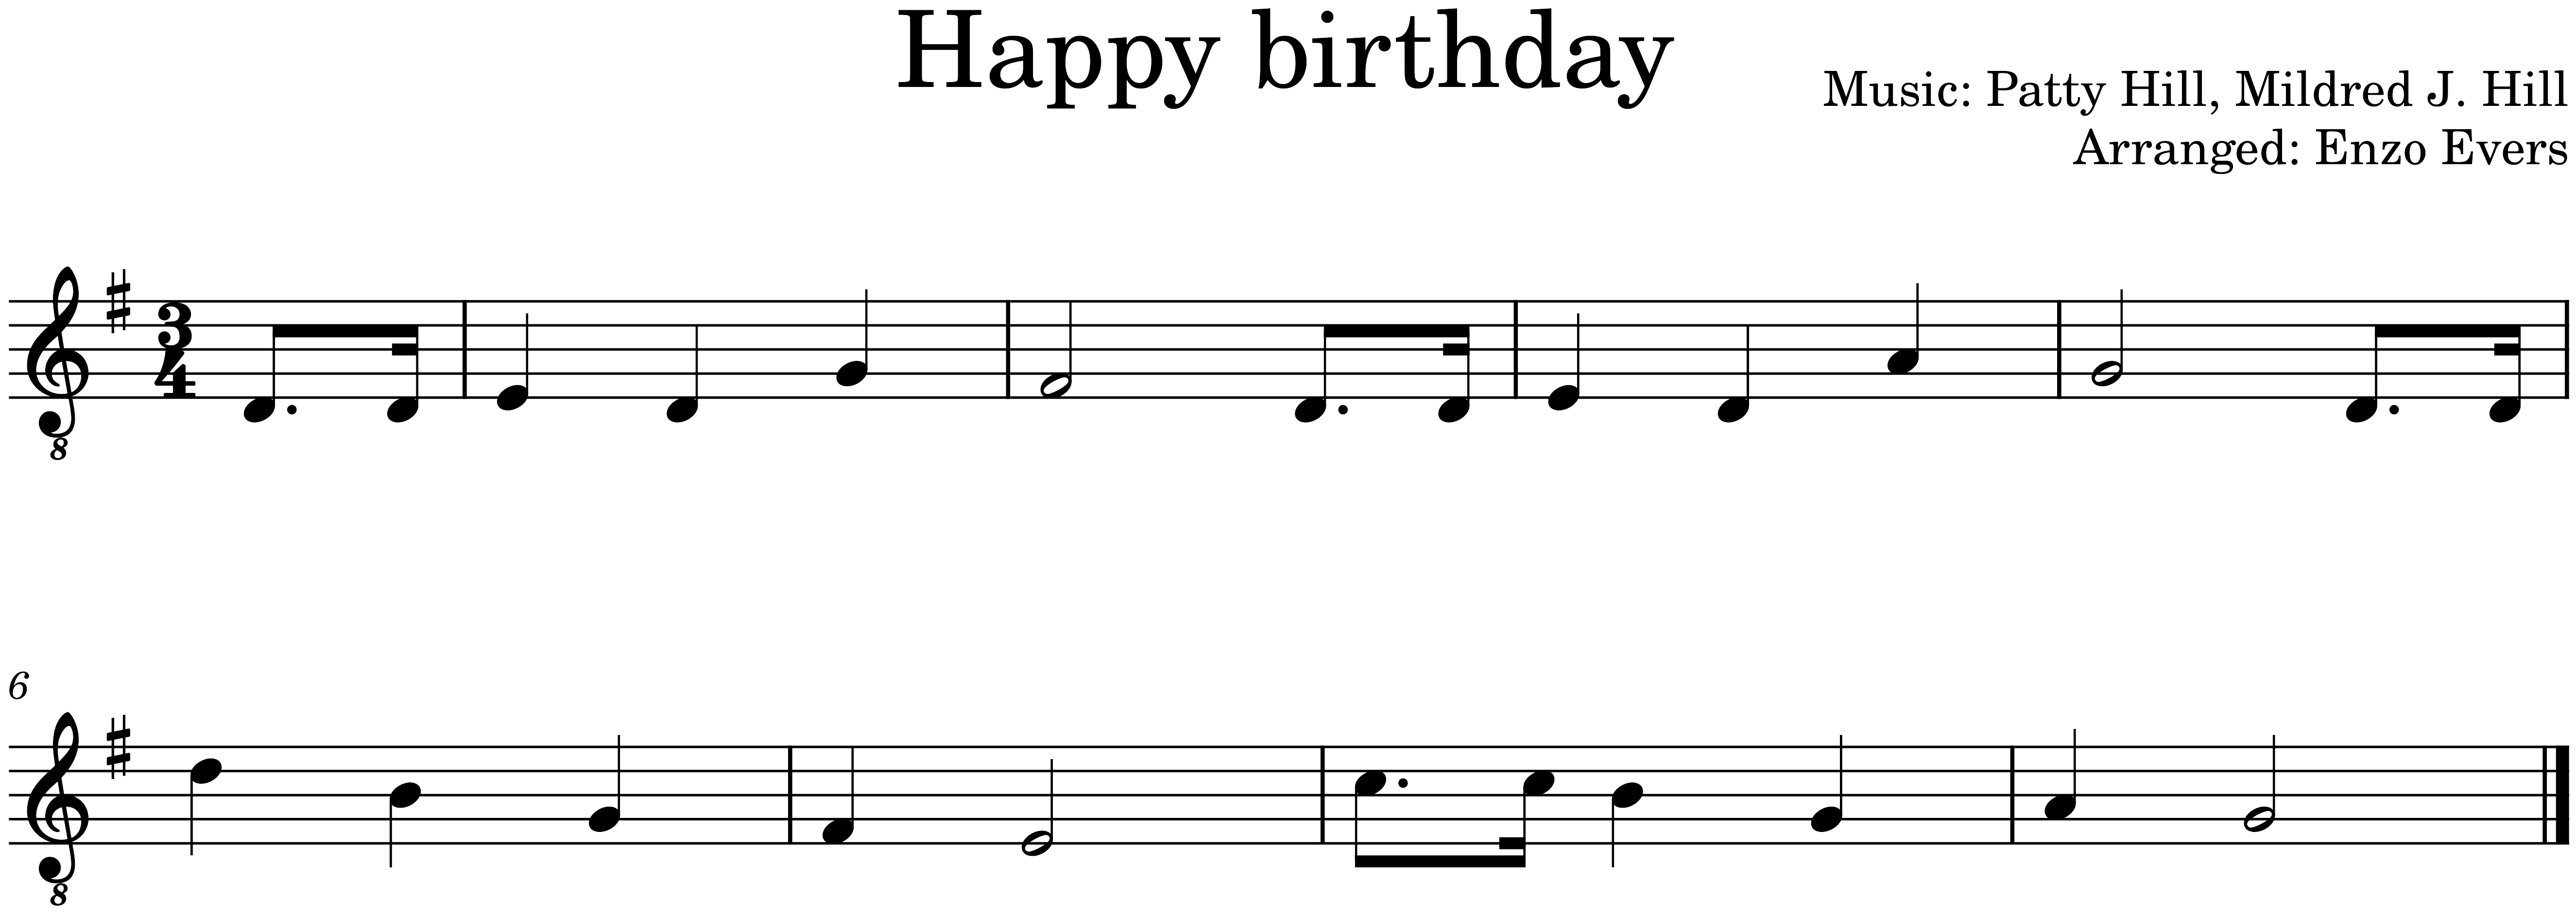
\includegraphics[width=\textwidth]{../../MuseScore/Guitar/GuitarHappyBirthdaySharps.png}
	\caption{Happy birthday with sharps}
	\label{fig:guitar_happy_birthday_sharps}
\end{figure}

In \autoref{fig:guitar_cest_la_vie_intro_chorus_melody} there are two song-wide sharps. The F and the C.

\begin{figure}[h]
	\centering
	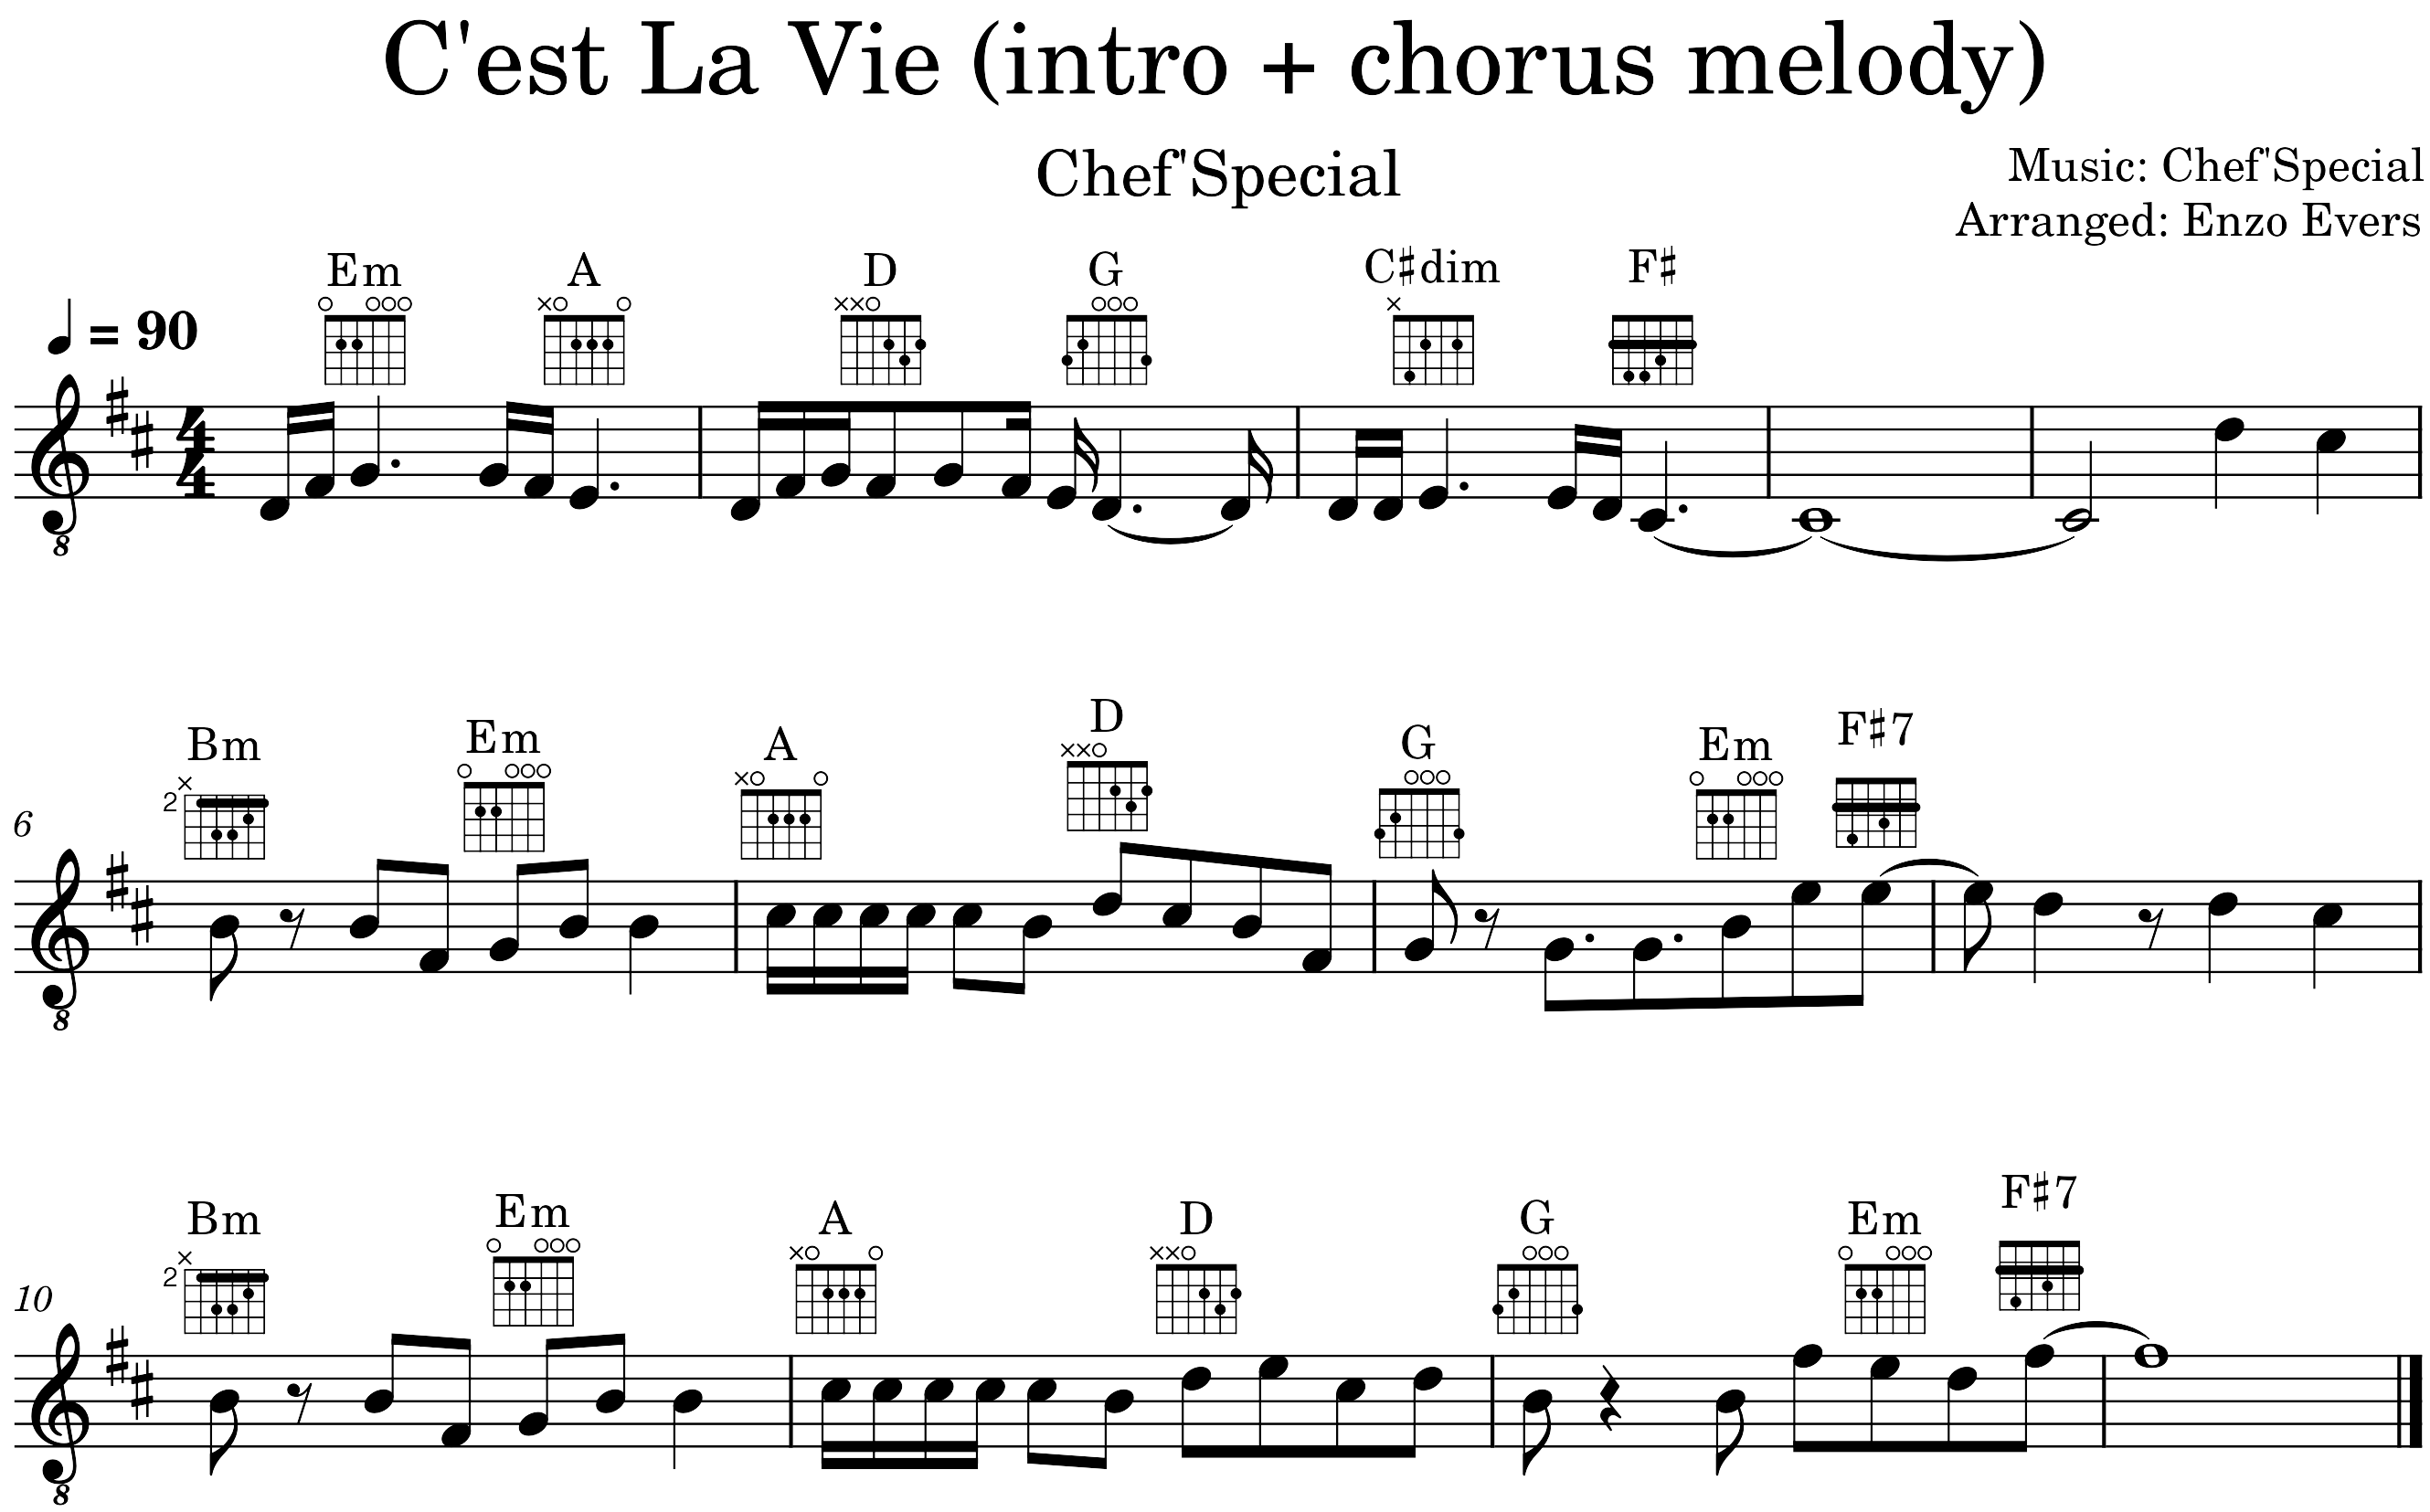
\includegraphics[width=\textwidth]{../../MuseScore/Guitar/GuitarCestLaVieChefSpecial_IntroChorus.png}
	\caption{C'est La Vie - Chef'Special (intro + chorus melody)}
	\label{fig:guitar_cest_la_vie_intro_chorus_melody}
\end{figure}

In Hedwig's Theme (see the next page) you will see the usage of sharps, flats, naturals and music-wide sharps. It uses the same music-wide F$\sharp$ as Happy birthday.

To better help you learn the position of these notes there is an empty tablature staff added. You can fill this staff with the correct tabs to help you learn.

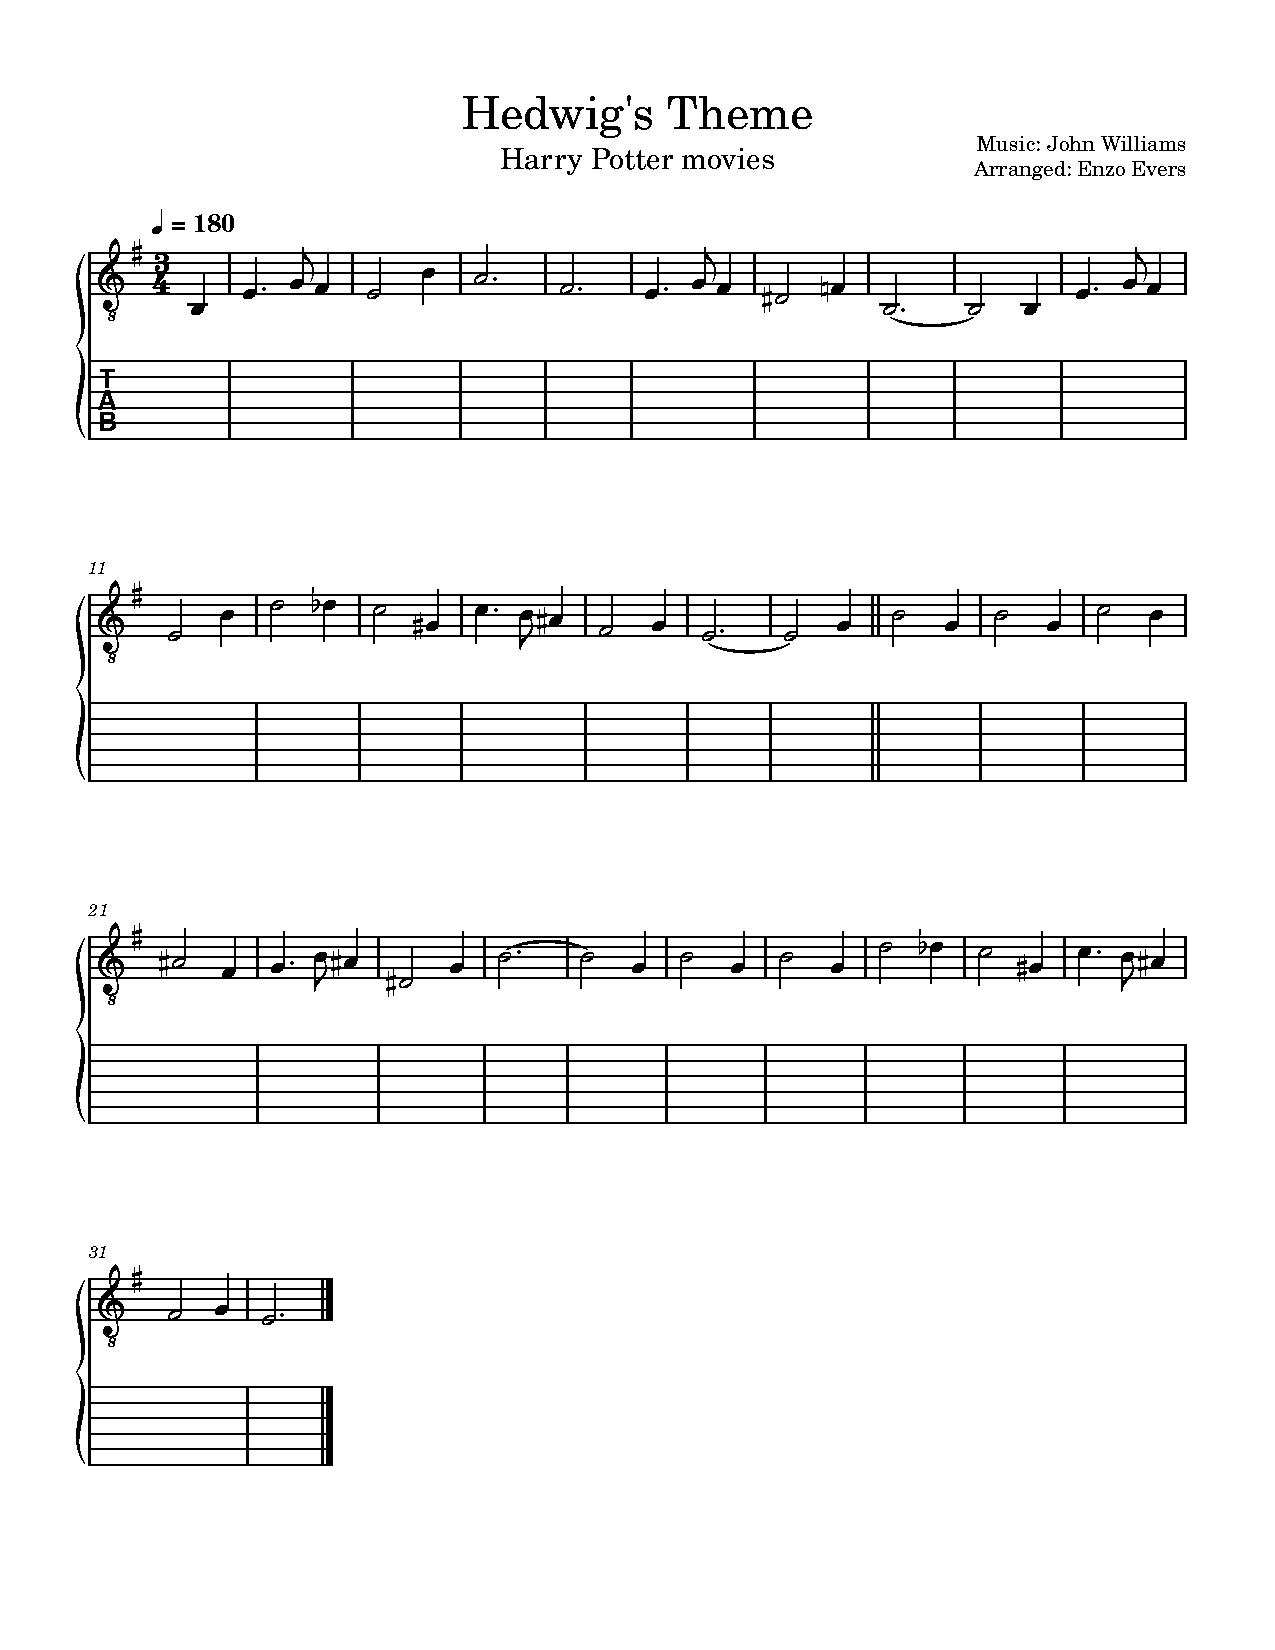
\includepdf[pages=-,pagecommand={\thispagestyle{headings}}]{../../MuseScore/Guitar/GuitarHarrysPotterHedwigsTheme.pdf}

The next classical piece introduces a couple new things

First it introduces the high A and B notes (\autoref{fig:guitar_notes_high_a_b}). Previously it was already explained how the notes below the staff lines can be determined. The same holds for notes above the staff.

\begin{figure}[h]
	\centering
	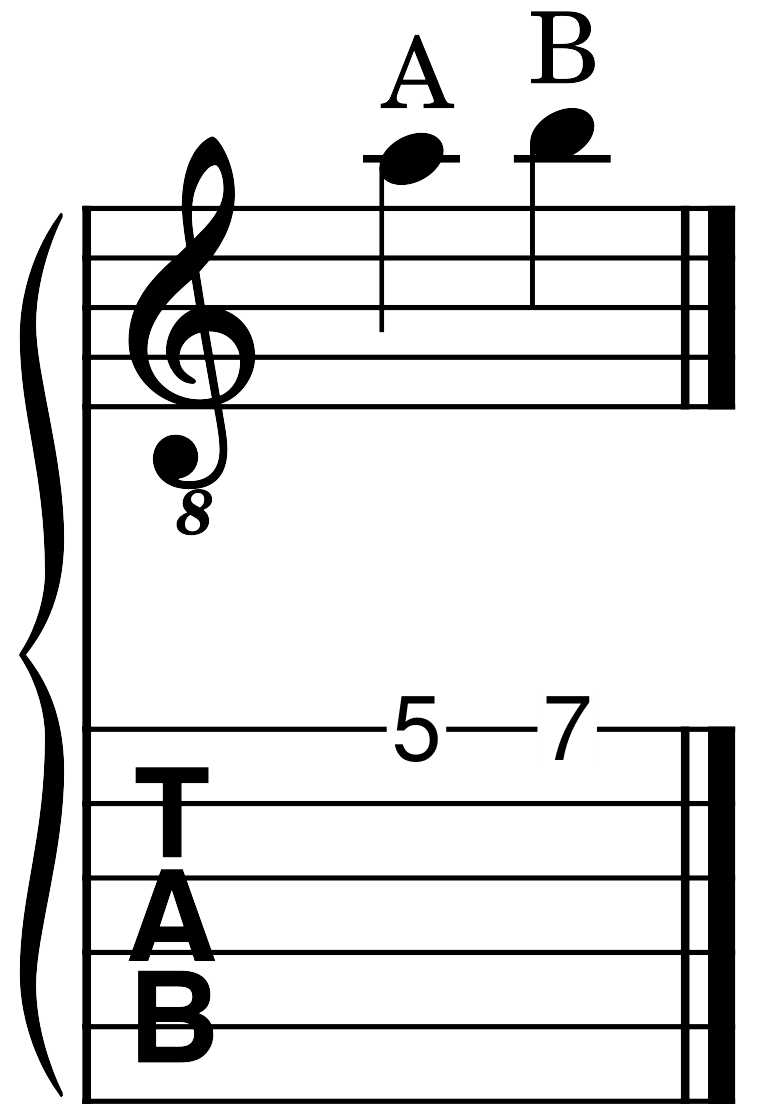
\includegraphics[height=0.12\textheight]{../../MuseScore/Guitar/GuitarNotesHighAB.png}
	\caption{The high A and B notes}
	\label{fig:guitar_notes_high_a_b}
\end{figure}

The other new symbol is the repeat symbol as seen in \autoref{fig:guitar_repeat_symbol}. When you come to the end of the measure that has the right side of the repeat symbol, you go back to the left repeat symbol. When you come to the right repeat symbol again, you will just play further this time.

\begin{figure}[h]
	\centering
	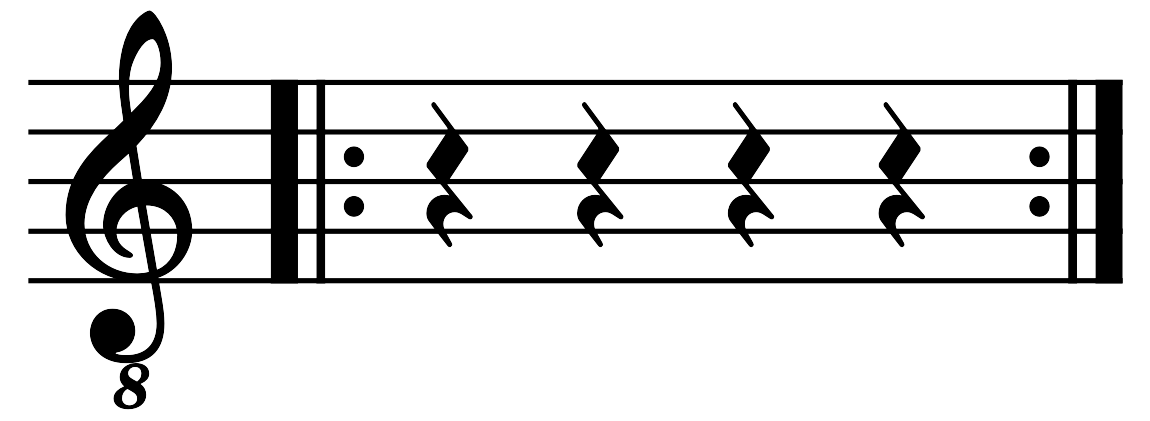
\includegraphics[height=0.05\textheight]{../../MuseScore/Guitar/GuitarRepeatSymbol.png}
	\caption{The repeat symbol}
	\label{fig:guitar_repeat_symbol}
\end{figure}

Another thing you will see in this song is that there are two parts. One for the melody and one for the bass line. This sheet music is meant to be played by two people together.

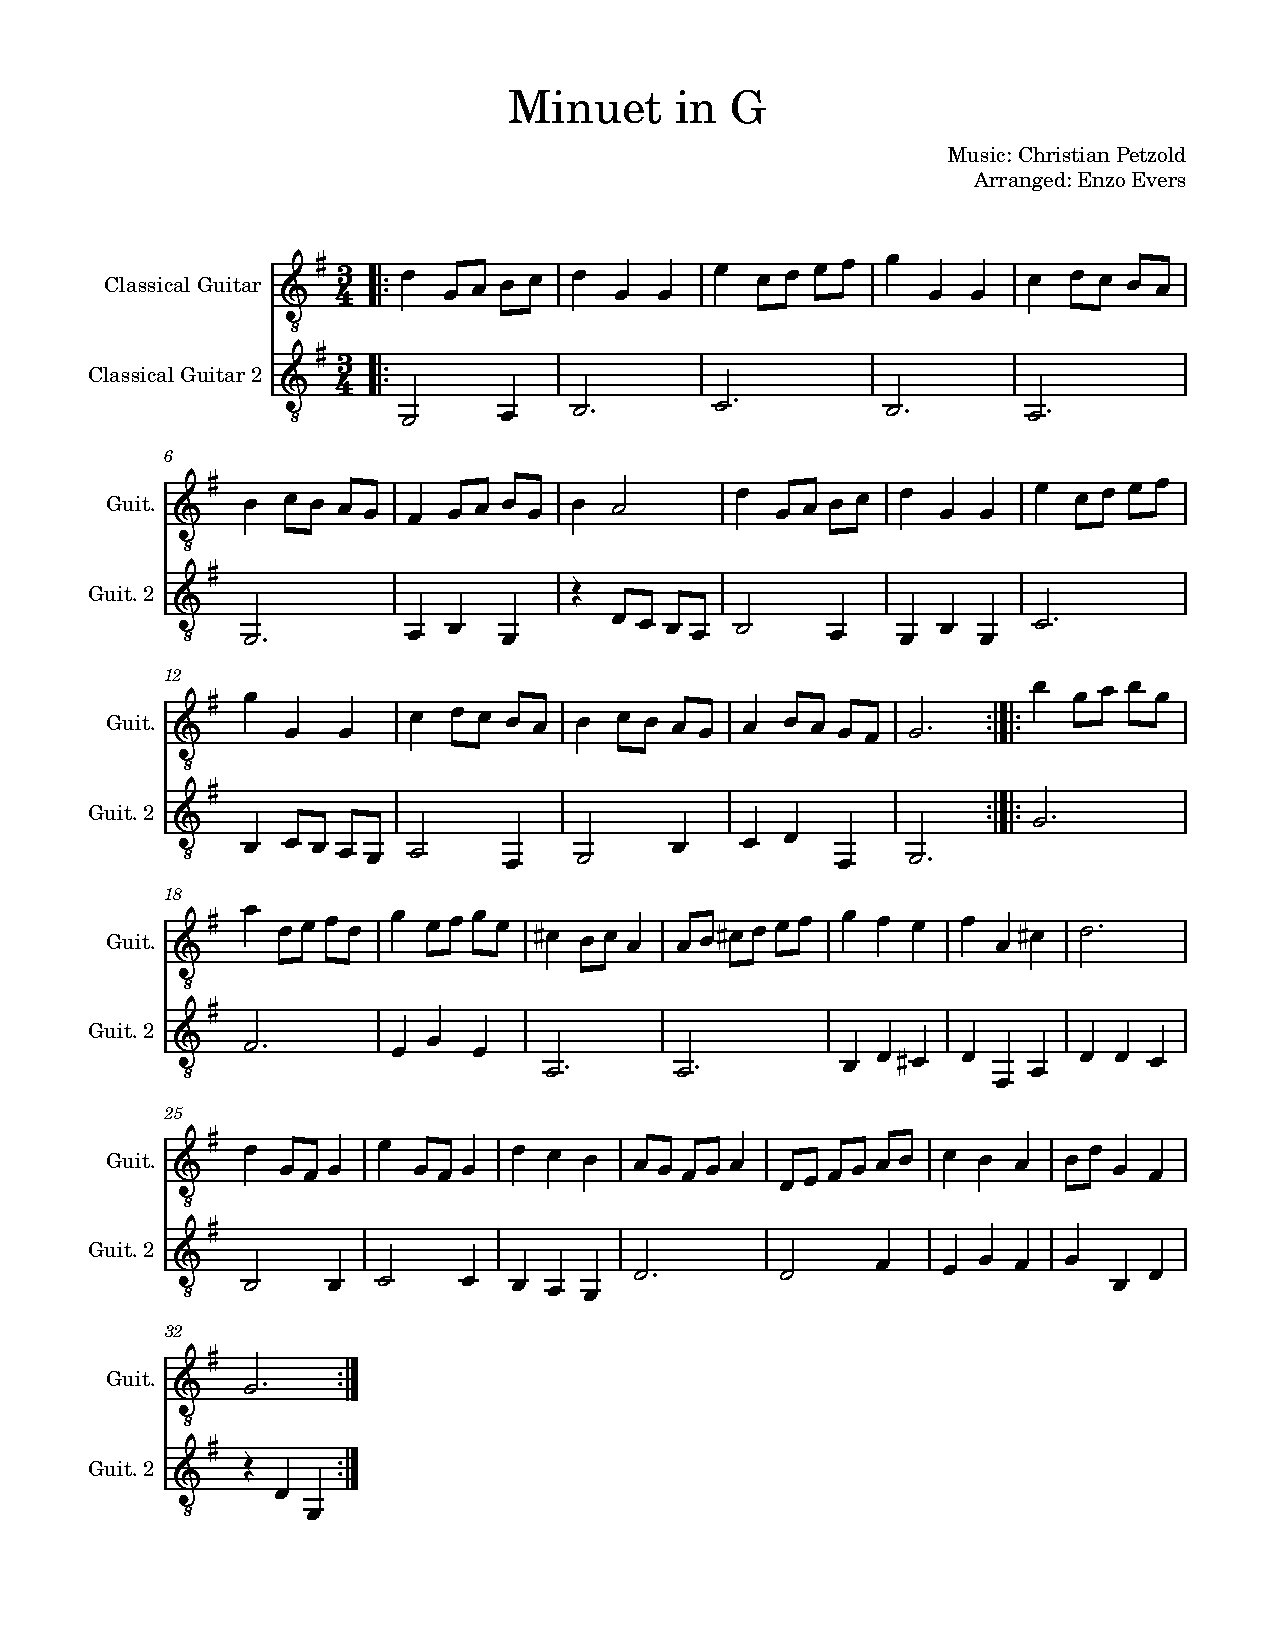
\includepdf[pages=-,pagecommand={\thispagestyle{headings}}]{../../MuseScore/Guitar/GuitarMinuetInG.pdf}

As promised, the whole Tetris tune would be played when we learned about sharps. So here it is (\autoref{fig:guitar_tetris_full}).

This also introduces the \textbf{D.C. al Fine} term. The "D.C. al Fine" term means to go back to the beginning of the music piece and play until you see the "Fine" text. Then the music is finished. Here "D.C." means "Da Capo" and is Italian for "from the beginning".

\begin{figure}[h]
	\centering
	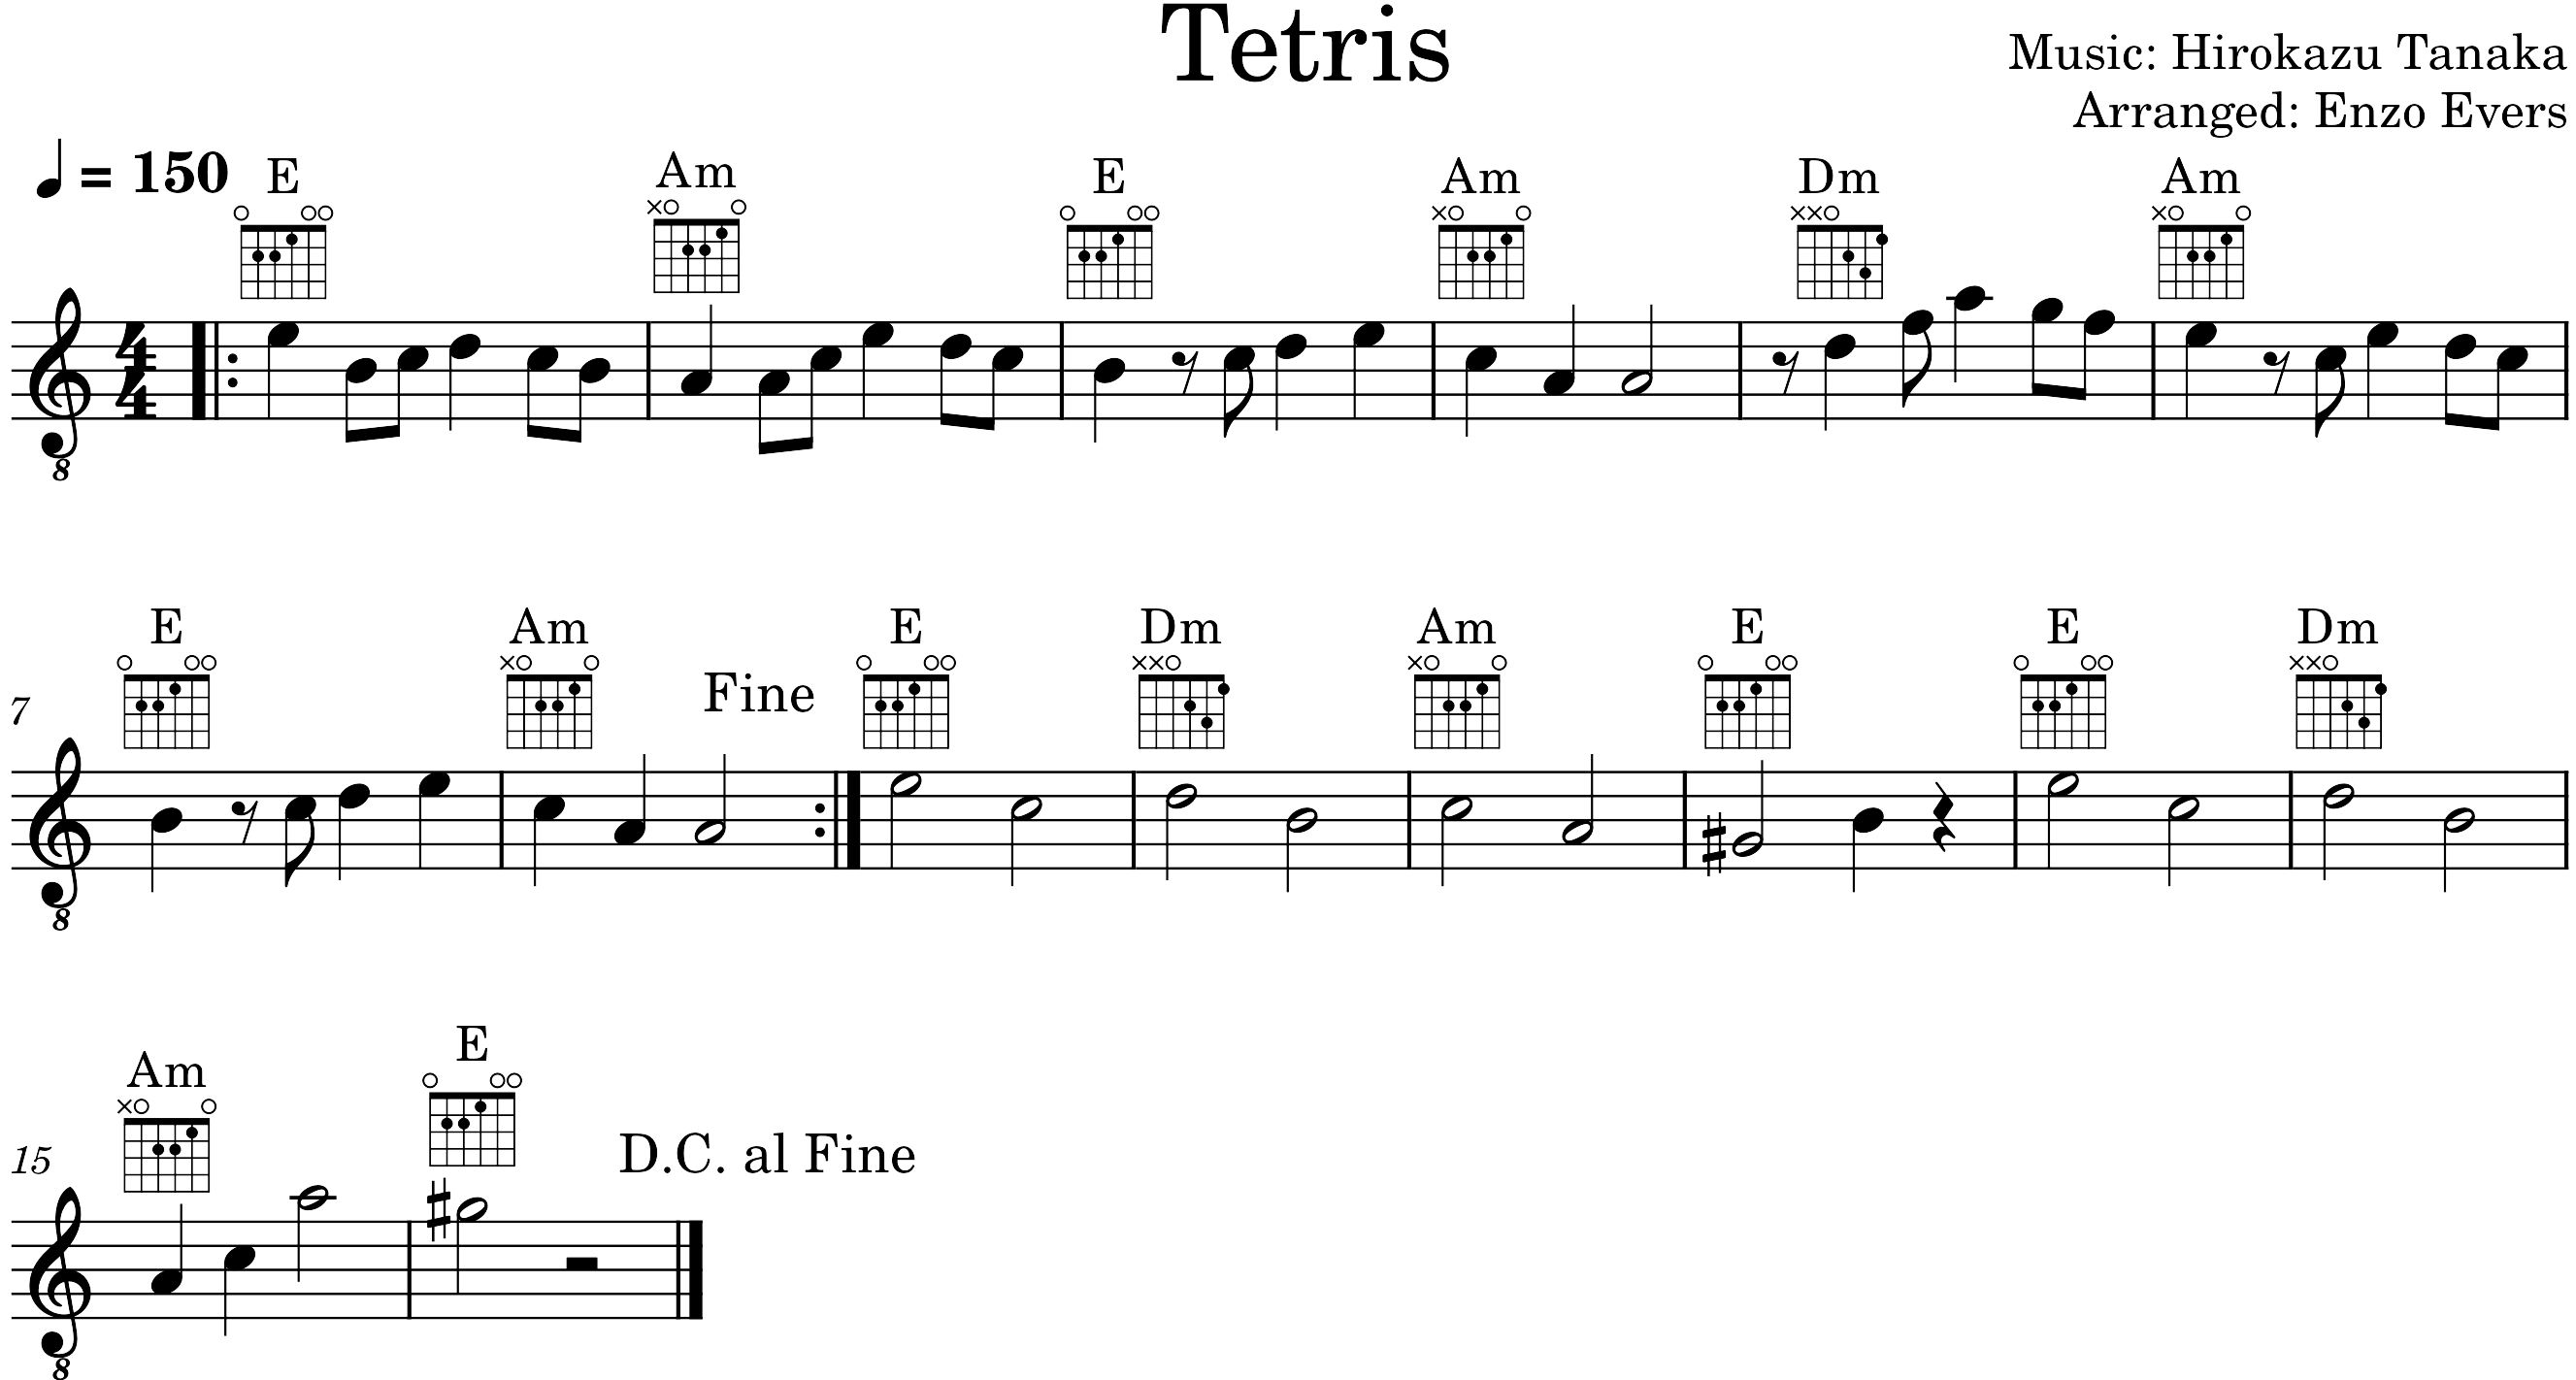
\includegraphics[width=\textwidth]{../../MuseScore/Guitar/GuitarTetrisFull.png}
	\caption{Tetris tune (full)}
	\label{fig:guitar_tetris_full}
\end{figure}

In the song "He's a pirate" (see the next page) from the "Pirates of the Caribbean" movies there is one new note. The High C (\autoref{fig:guitar_note_high_c}).

\begin{figure}[h]
	\centering
	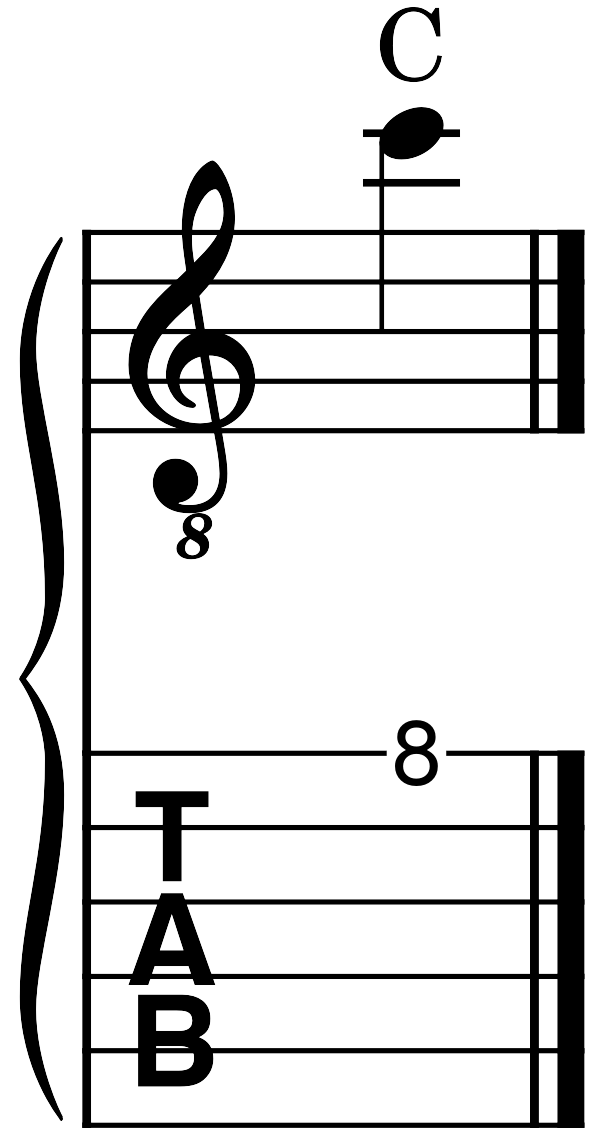
\includegraphics[height=0.12\textheight]{../../MuseScore/Guitar/GuitarNotesHighC.png}
	\caption{The high C note}
	\label{fig:guitar_note_high_c}
\end{figure}

This song has a song-wide flat B.

This song also introduces the concept of playing in a different position. Measure 32 - 39 are played from the 3rd position, and from measure 40 till the end you are playing in the 5th position. What this means is that you take the 3rd and 5th fret respectively as the 'starting' point. Imagine that the frets before that don't exist. This forces you to learn where identical pitched notes can be played on the fretboard.

The benefit of these positions is that you don't have to fly with your hand all over the fretboard. Instead, by utilizing the correct finger positions you can keep your hand in one position.

To help you, think about the relative tuning diagram from the beginning (\autoref{fig:guitar_relative_tuning}) and the interval of each fret (a semitone) together with how these steps relate do the different notes (\autoref{sec:fretboard_introduction}). 

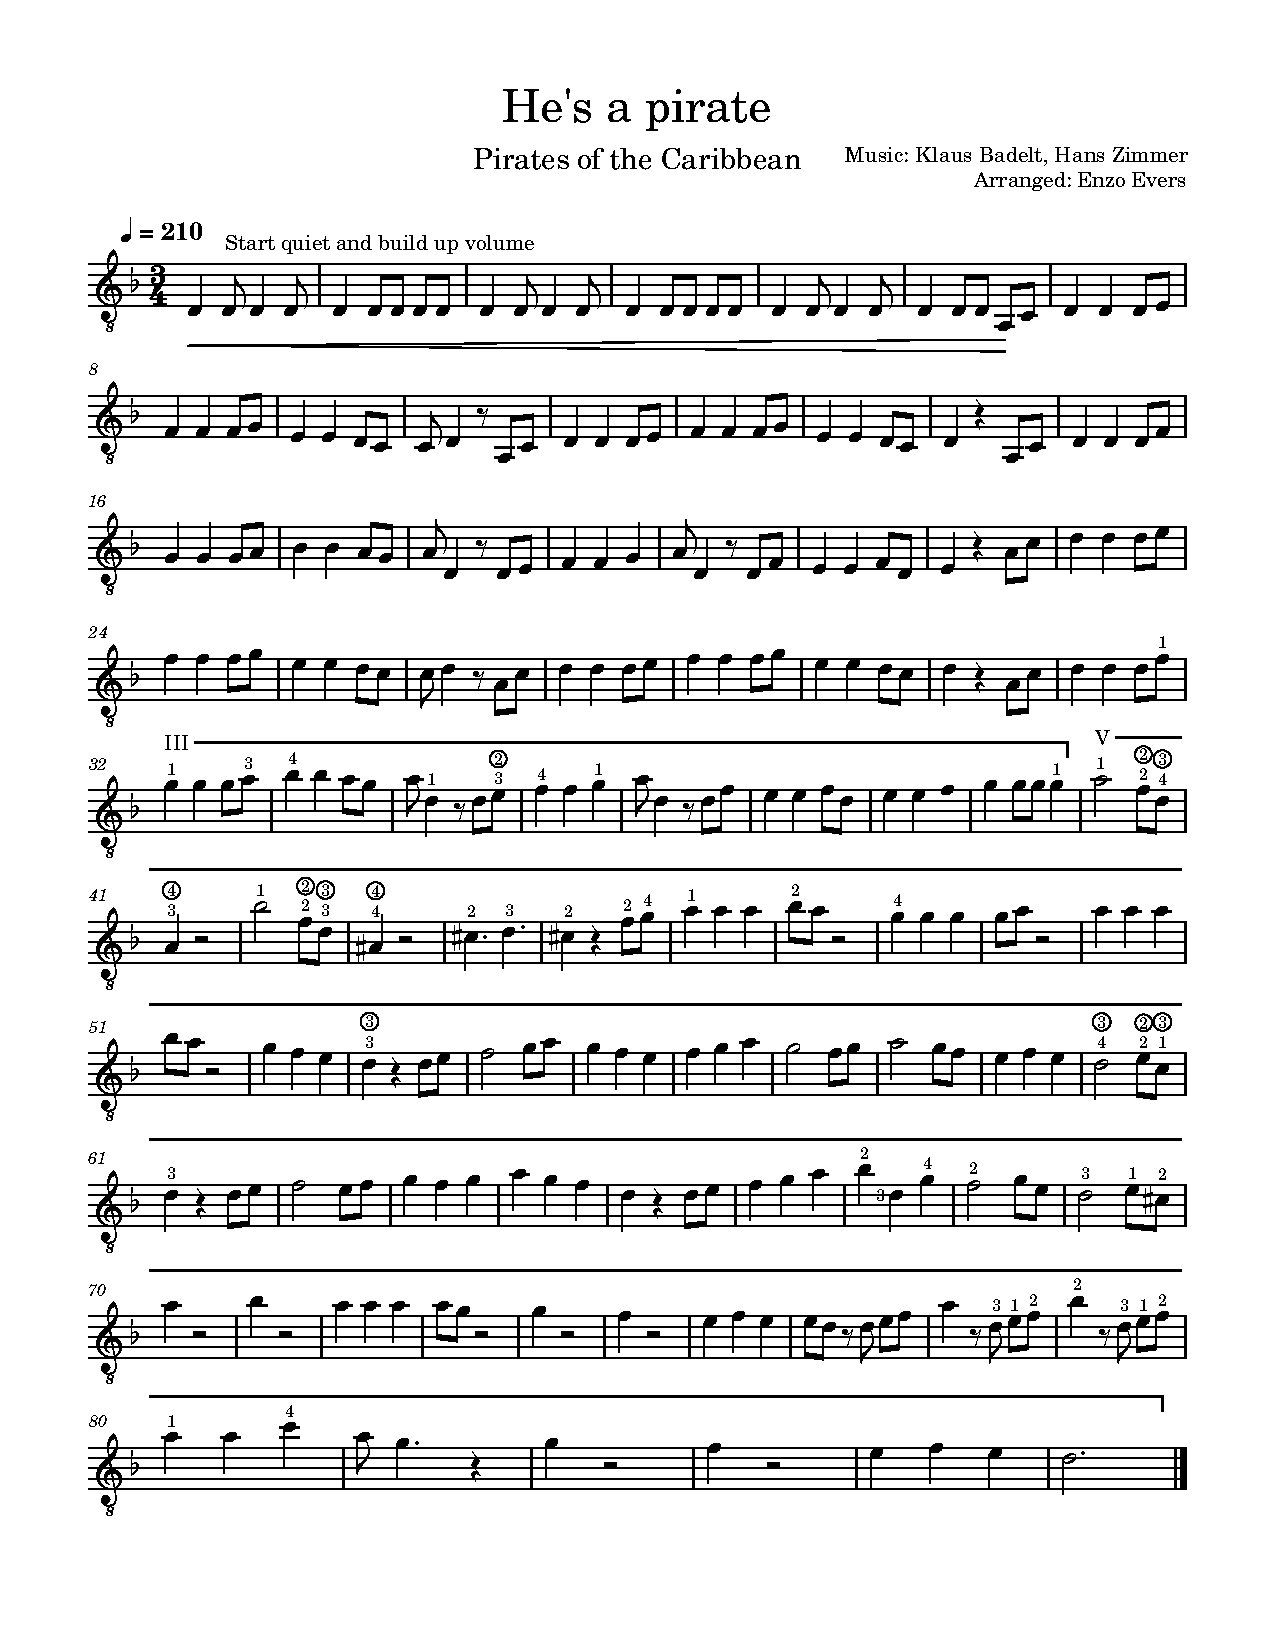
\includepdf[pages=-,pagecommand={\thispagestyle{headings}}]{../../MuseScore/Guitar/GuitarHesAPirate.pdf}

